%%
%% Beuth Hochschule für Technik -- Masterarbeit
%%
%% Hauptdokument
%%
%--------------------------------------------------------------%

\documentclass[11pt, a4paper,twoside]{report}
\usepackage[abgabe]{bhtThesis}
\typeout{Masterarbeit}

\usepackage{graphicx}
\usepackage{hyperref}

\usepackage{blindtext}
\usepackage{listings}
\usepackage{color}

\lstset{
	literate =	{ö}{{\"o}}1
				{ä}{{\"a}}1
				{ü}{{\"u}}1
				{Ö}{{\"O}}1
				{Ä}{{\"A}}1
				{Ü}{{\"U}}1
				{ß}{{\ss}}1
}
\usepackage{trsym}
\usepackage{bytefield}
\usepackage{longtable}
\definecolor{light-gray}{gray}{0.90} %Code Hintergundfarbe
\definecolor{darkBHT}{rgb}{0,0.5882,0.5529}
\setlength{\parskip}{6pt}
\setlength{\parindent}{0pt}
\definecolor{lightgray}{rgb}{.9,.9,.9}
\definecolor{darkgray}{rgb}{.4,.4,.4}
\definecolor{purple}{rgb}{0.65,0.12,0.82}


%##################################################################
%Pfad zu den Bildern
%##################################################################
\graphicspath{
	{pictures/}%,
	{4_Loesungsansatz/},
%	{5_Systementwurf/pictures/}
}



%format for program code
\lstset{language=Java,
				backgroundcolor=\color{white},
				tabsize=2,
				breaklines=true,
				numbers=left,
				numbersep=0pt,
				numberstyle=\color{gray},
				basicstyle=\ttfamily\color{black}\small,
				keywordstyle=\color{black},%\bfseries,
				commentstyle=\color{gray}\slshape,
				identifierstyle=\color{black}
		}


		
\begin{document}
%##################################################################
% Titelpage
%##################################################################
\pagestyle{fancy}
\begin{titlepage}
	\begin{center}
		\Large
		Beuth Hochschule für Technik Berlin
		\textcolor{darkBHT}{\rule{\textwidth}{0.2cm}} \\
		\vspace{2 cm}
		
		\Large		
		\textbf{Masterarbeit}
		
		\huge
		\textbf{Variantenspezifische Abhängigkeitsregeln und Testfallgenerierung in TESTONA\\}

		\vspace{2cm}
		
		\begin{figure}[htbp]
			\centering 
			
\includegraphics[width=7cm]{BHT-Logo-Basis.pdf}  
		\end{figure}

\Large
Fachbereich VI - Technische Informatik - Embedded Systems
		
		\vspace{1cm}		

		\begin{figure}[htbp]
			\centering 
			
\includegraphics[scale=0.3]{BernerMattner_Logo.pdf}  
		\end{figure}		
		
		\vspace{1cm}
		
		\begin{center}
		Eingereicht am: \today
		\end{center}
		
		\begin{tabular}{lll}
			Erstprüfer    &: &Prof.  Dr. rer. nat. Macos \\
			Zweitprüfer   &: &Prof.  Dr.-Ing. Höfig\\
			Eingereicht von&: &Matthias Hansert \\
			Matrikelnummer&:  &s791744\\
			Email-Adresse &: &matthansert@gmail.com\\
		\end{tabular}
		
		\date{\today}
		
	\end{center}
	\vfill
	\textcolor{darkBHT}{\rule{\textwidth}{0.2cm}}
	\normalsize
	
	\newpage
\end{titlepage}

%one empty page before table of contents
\newpage
\thispagestyle{empty}
\mbox{}
\newpage
\thispagestyle{empty}
\mbox{}


%##################################################################
% Dankessage
%##################################################################


\begin{center}


\begin{LARGE}
Dankessage
\end{LARGE}




\end{center}



%one empty page before table of contents
\newpage
\thispagestyle{empty}
\mbox{}

%##################################################################
% Inhaltsverzeichnis
%##################################################################
\pagenumbering{Roman}
\tableofcontents
%one empty page after table of contents
\newpage
\thispagestyle{empty}
\mbox{}

%##################################################################
% Die Kapitel
%##################################################################

\pagenumbering{arabic}

\chapter{Einleitung}\label{chp:einleitung}
\paragraph{}
%Gefordert ist......
Ziel dieser Masterarbeit ist die Erweiterung und Verbesserung des Berner \& Mattner Werkzeuges TESTONA. Dieses Programm bietet Testern ein Werkzeug für eine strukturierte und systematische Ermittlung von Testszenarien\footnote{Kombination mehrerer Testfälle mit dem Ziel, komplexeren Sachverhalten zu überprüfen.}\cite{TESTONA}. Im Kapitel \ref{sec:Testona} wird weiteres zu diesem Programm und die Funktionsweise erläutert.\\

Die Erweiterung des Programmes besteht aus verschiedenen Themen. Ein Thema davon behandelt die Testfallgenerierung und die jeweilige Testabdeckung\footnote{(engl. Test Coverage bzw. Code Coverage) das Verhältnis an tatsächlich getroffenen Aussagen eines Tests gegenüber den theoretisch möglich treffbaren Aussagen. Tests werden anhand der Spezifikation einer zu testenden Software-Einheit definiert.\cite{TestAbdeckung}}. Hier soll garantiert werden, dass bei einer automatischen Testfallgenerierung, eine höchstmögliche Testabdeckung erzielt wird.\\

Die Testfallgenerierung wird in dieser Arbeit beeinflusst, indem die Produktvarianten stärker betrachten werden. Verschiedene Varianten beinhalten verschiedene Parameter und Produktkomponenten (Eigenschaften). Die Parameterwerte definieren auch verschiedene Produktvarianten. Durch das Add-On MERAN für die Anforderungsmanagementsoftware \glqq IBM Rational DOORS\grqq~ können Anforderungen und Varianten direkt in  TESTONA importiert werden. Dabei sollen automatisch die Parameterwerte zur jeweiligen Produktvariante zugeordnet werden. Aus diesem Grund kann es zu Konflikten bei der Testfallgenerierung kommen, bzw. inkohärente Testfälle können auftreten.\\

Um solche Probleme zu vermeiden oder zu umgehen, gibt TESTONA den Testern die Möglichkeit Abhängigkeitsregeln anzulegen. Hier können Anfangsbedingungen sowie Sonderbedingungen definiert werden. Dabei muss wiederum beachtet werden, dass die Produktvarianten nicht verletzt werden. Weiteres zu den Themen und Begriffen wird im Kapitel \ref{chp:fachlichesumfeld} verdeutlicht.\\

Im Kapitel \ref{chp:aufgabenstellung} wird die Aufgabe dieser Masterarbeit genauer erläutert und in den Kapiteln \ref{chp:loesungsansatz} und \ref{chp:systementwurf} jeweils eine Lösung vorgeschlagen und implementiert.

%#######################################################################################

\chapter{Aufgabestellung}\label{chp:aufgabenstellung}
\paragraph{}

Ziel dieser Masterarbeit ist die Verbesserung der Testfallgenerierung und der Testabdeckung bei mehreren Produktvarianten, die Ersetzung von Parametern, die Prozessoptimierung sowie die Handhabung für den Benutzer in der TESTONA-Umgebung. Jedes Produkt kann unterschiedliche Produktvarianten beinhalten und jede Variante besteht aus unterschiedlichen Komponenten mit unterschiedlichen Parametern. In Abhängigkeit von der ausgewählten Variante sollen bei der Testfallgenerierung die dazugehörigen Komponenten berücksichtigt werden und die erzeugten Testfälle dargestellt werden. Besonders zu beachten sind dabei die definierten Abhängigkeitsregeln sowie die darauf bezogene Testabdeckung.\\

Abhängigkeitsregeln werden definiert um redundante Testfälle zu vermeiden, bzw. um Vorbedingungen für die Testfälle zu erstellen. Da Varianten verschiedene Baumelemente beinhalten, kann es dazu kommen, dass Baumelemente für Abhängigkeitsregeln nicht vorhanden sind. Dadurch könnte TESTONA bei der Testfallgenerierung die Testabdeckung verfälschen, indem die Gültigkeit eines Testfalles nicht garantiert werden kann. Um dieses Problem zu umgehen, muss bei der Erzeugung von Abhängigkeitsregeln auf mögliche Konflikte hingewiesen werden. Für den Lösungsansatz gibt es verschiedene Thesen die analysiert werden müssen, um eine optimale Prozessoptimierung zu erreichen.\\

Um die Handhabung der Varianten bezogen auf die Testfälle und die Testgenerierung benutzerfreundlicher und effizienter zu gestalten, soll die Benutzung des Variantenmanagements durch einen Testingenieur untersucht werden. Resultierend aus den erworbenen Erkenntnissen wird das Lösungsdesign für eine Erweiterung des bestehenden Variantenmanagements in TESTONA konzipiert.\\

Einer der besonderen Eigenschaften von TESTONA ist die Kopplung mit Anforderungsspezifikationen die in IBM Rational DOORS definiert worden sind. Durch das DOORS Add-On MERAN können Anforderungen die in DOORS definiert sind, mit den zugehörigen Varianten verknüpft werden. Diese Varianten können durch eine erfolgreiche Anmeldung bei DOORS (über die TESTONA Oberfläche) und ein gezieltes Auswählen der gewünschten Varianten in TESTONA eingebunden werden. Hierbei sollen die in den Anforderungen definierten Parametern (z.B. eine Geschwindigkeit oder die Anzahl der Türen eines Autos) mit gespeichert werden. Im Klassifikationsbaum soll je nach ausgewählter Variante (z.B. der Name von Klassen) mit dem entsprechenden Wert ersetzt werden. Andere Lösungsmöglichkeiten werden noch untersucht.\\

Der derzeitige Varianten-Management-Ansatz in TESTONA ist nicht in der Lage für die Testfallgenerierung zwischen verschiedene Varianten zu unterscheiden. Zwar werden durch die Perspektive „Variant Management“ verschiedene Varianten unterschieden, aber die Testfälle müssen manuell mit den jeweiligen Varianten verknüpft werden. Im Falle einer automatischen Testfallgenerierung werden auch ungültige Baumelemente betrachtet (siehe Abbild \ref{ttn.gruen} und \ref{ttn.rot}). Um dies zu vermeiden muss der Testingenieur einzelne Generierungsregeln anlegen. Dieser Vorgang soll automatisiert und von TESTONA übernommen werden. Dabei gibt es verschiedene Betrachtungsweisen und mehrere Lösungswege. Die erworbenen Kenntnisse des Testingenieurs über die Benutzung des Variantenmanagements sind entscheidend für die Lösung. Bei der Lösung ist zu beachten, dass eine komplette Testfallabdeckung garantiert werden muss.\\


\begin{figure}[h]
  \begin{center}
    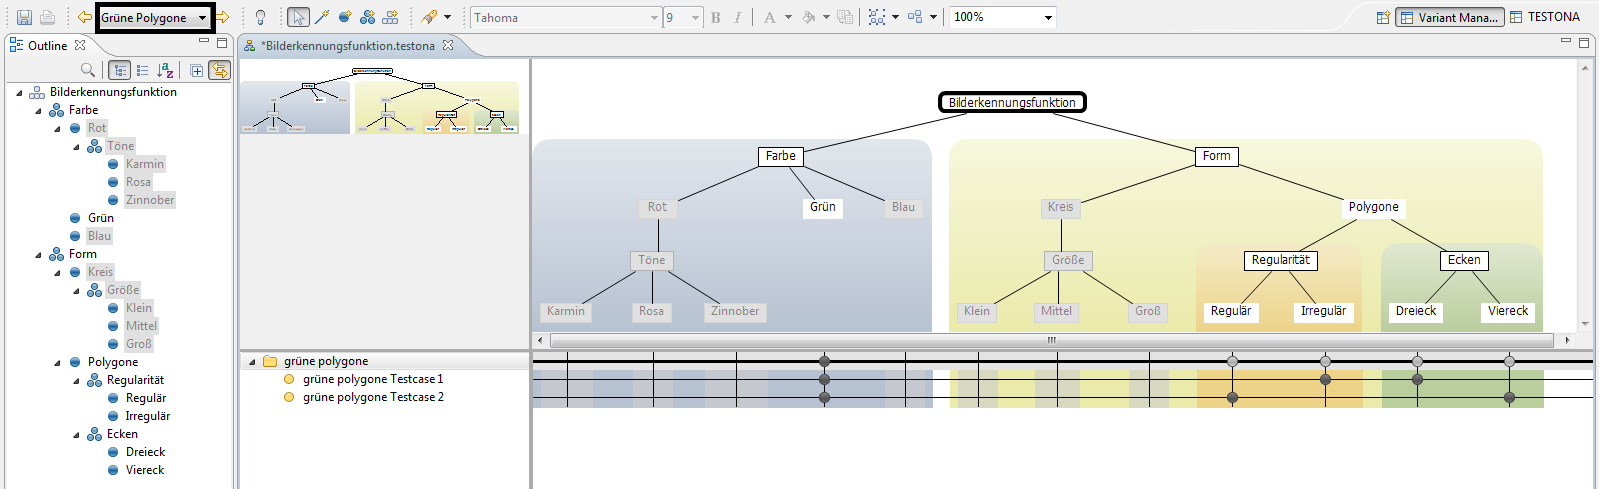
\includegraphics[scale=0.35]{gruenePolygone_DE.png}
  		  \caption{Richtige Auswahl der Klassen und Klassifikationen für die Testfallgenerierung}
     \label{ttn.gruen}
  \end{center}
\end{figure}


\begin{figure}[h]
  \begin{center}
    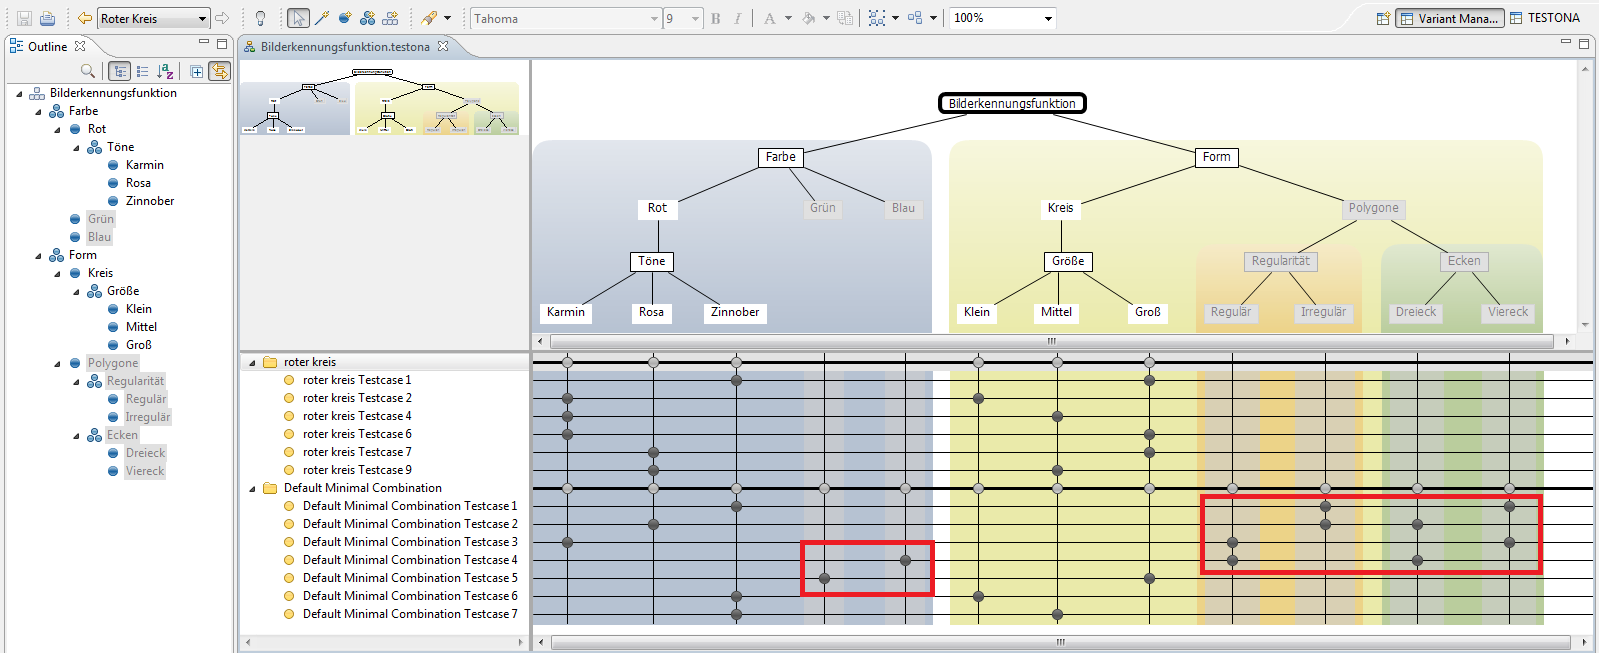
\includegraphics[scale=0.35]{roterKreis_DE.png}
  		  \caption{Ungültige Auswahl der Klassen (Grün und Blau) und Klassifikationen (Regularität und Ecken) für die Testfallgenerierung}
     \label{ttn.rot}
  \end{center}
\end{figure}



\chapter{Fachliches Umfeld}\label{chp:fachlichesumfeld}

%#######################################################################################
%#######################################################################################
\section{TESTONA}\label{sec:Testona} 
\paragraph{}

Mit TESTONA wird dem Tester ein Tool angeboten, um signifikante Testszenarien und -umfänge strukturiert zu bestimmen. Mit dem Programm können komplette Testspezifikationen schnell und einfach generiert werden und überflüssige Testfälle vermieden werden. Bei Bedarf gibt es die Möglichkeit automatische generierte Testspezifikationen und Testfälle bequem mit Anforderungen durch Add-Ons an Standard-Werkzeugen zu verlinken (siehe \ref{sec:DOORS}). Somit werden robuste Schnittstellen für ein komfortables Anforderungs- und Testmanagement erzeugt. Ein sehr wichtiger Aspekt von TESTONA ist, dass es Branchen-unabhängig ist. Das heißt ein Tester kann TESTONA im jedem Fachgebiet benutzen, nicht nur bei Software- oder Funktionstests.\\

Mehr zu Testfällen und der Arbeitsweise dieses Programms werden in den nächsten Kapiteln erläutert, wie zum Beispiel die anerkannte Klassifikationsbaum-Methode.



%#######################################################################################
\subsection{Klassifikationsbaum-Methode}\label{ssec:KM}
\paragraph{}
1993 entwickelten K. Grimm und M. Grochtmann die Klassifikationsbaum-Methode zur Ermittlung funktionaler Blackbox-Tests im Bereich von eingebetteter Software. Die Methode wurde im Forschungslabor von Daimler-Benz in Berlin als Weiterentwicklung der Category-Partition Method (CPM) erforscht. Gegenüber CPM hat die Klassifikationsbaum-Methode eine graphische Baum-Darstellung und hierarchische Verfeinerungen für implizite Abhängigkeiten. Als Werkzeug wurde der \glqq Classification Tree Editor\grqq~ (CTE) \footnote{Entwickelt von Grochtmann und Wegener\cite{TestCaseDesign}. Bei Berner  \& Mattner aus rechtlichen Gründen zu TESTONA umbenannt} programmiert und unterstützt Partitionierung und Testfallgenerierung. Das Werkzeug von CPM konnte nur Testfälle generieren ohne Bestimmung der Testaspekte\cite{ClassificationTrees}.

 Diese Methode besteht aus zwei wichtigen Schritten:
\begin{itemize}
\item Bestimmung der Klassifikationen (testrelevante Aspekte) und Klassen (mögliche Ausprägungen).
\item Erzeugung von Testfällen aus Kombinationen von unterschiedlichen Klassen für alle Klassifikationen
\end{itemize}

Ansatzpunkt sind die funktionalen Anforderungen (siehe \ref{sec:DOORS}) eines zu testenden Objekts. Um die Testfälle zu definieren und zu erzeugen, folgt die Methode dem Prinzip des kombinatorischen Testentwurfs \cite{KlassifikationsbaumMethode}. Dieses Prinzip hilft bei der Detektierung von Fehlern in frühen Schritten des Testvorgangs. Nicht jeder einzelne Parameter steuert einen Fehler bei, eher werden Fehler durch die Interaktion verschiedener Parameter verursacht. Betrachten wir ein einfaches Beispiel. Ein Programm soll auf Windows oder Linux laufen, unter Verwendung eines AMD oder Intel Prozessors und mit Unterstützung des IPv4 oder IPv6 Protokolls. Das ergibt intuitiv acht verschiedene Testfälle ($2^{3} = 8$ Möglichkeiten, siehe Abbildung \ref{ttn.no_kombi}).\\

\begin{figure}[h]
  \begin{center}
    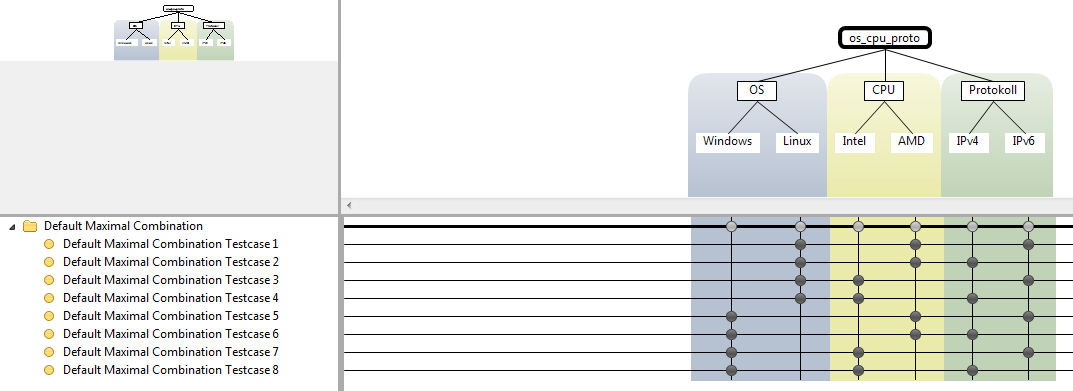
\includegraphics[scale=0.5]{os_cpu_proto_max_kombinatorik.png}
  		  \caption{Baum und Testfälle ohne Kombinatorik}
     \label{ttn.no_kombi}
  \end{center}
\end{figure}


Verwenden wir dafür den kombinatorischen Testentwurf \glqq paarweise Kombination\grqq~ (in Testona: \textit{pairwise(OS, CPU, Protokoll)} ), hätten wir nur vier Testfälle (siehe Tabelle \ref{table:4TestCases}). Durch diese Methode werden alle Kombinationspaare der Parameter mindestens durch einen Testfall abgedeckt\cite{CombinatorialSoftTesting}.\\

\begin{table}[h]


\begin{center}
	\begin{tabular}{|r||c|c|c|}
	 \hline
	 No. &OS &CPU &Protokoll\\
	 \hline \hline
	 1. &Linux &AMD &IPv6\\
	 \hline
	 4. &Linux &Intel &IPv4\\
	 \hline
	 5. &Windows &AMD &IPv6\\
	 \hline
	 8. &Windows &Intel &IPv4\\
	 \hline
	\end{tabular}
	
	\caption{Testfälle mittels paarweise Kombinatorik}
	\label{table:4TestCases}
\end{center}

\end{table}


Die Effizienz von diesem einfachen kombinatorischen Entwurf ist beim komplexeren System zu sehen. Hat ein System $20$ verschiedene Schalter und jeder Schalter $10$ verschiedene Einstellungen, so gibt es $10^{20}$ verschiedene Kombinationen. Durch Anwendung der paarweisen Kombination muss der Tester nur 180 Testfälle betrachten.\\

Verschiedene Experimenten haben gezeigt, dass durch die Verwendung von der paarweisen Kombinatorik die gleichen oder meistens mehrere Fehler entdeckt wurden, als mit der manuellen Testauswahl\footnote{Basierend auf funktionelle und technische Anforderungen, Use-Cases}. Paarweise Kombinatorik ist am meisten verbreitet, aber man kann durchaus auch die Drei-Wege-Kombinatorik verwenden. TESTONA implementiert standardmäßig Minimalabdeckung, Paarweise-, Drei-Wege- und N-Kombinatorik (wo N die maximale Anzahl an möglichen Parametern im Klassifikationsbaum ist, auch vollständige Kombinatorik genannt)\cite{CombinatorialSoftTesting}.\\




%#######################################################################################
\subsection{Testfälle und Testfallgenerierung}
\paragraph{}

Unter einem Testfall versteht man, die Beschreibung eines elementaren Zustands eines Testobjekts. Hierfür werden Eingangsdaten benötigt (Parameterwerte, Vorbedingungen) und ein erwarteter Folgezustand. Mit TESTONA werden Testfälle für eine vereinbarte Testspezifikation definiert. Laut IEEE 829 ist unter Testspezifikation zu verstehen: die Durchführung von

\begin{itemize}
\item\textbf{ Testentwurfsspezifikation}: verfeinerte Beschreibung der Vorgehensweise für das Testen einer Software
\item \textbf{Testfallspezifikation}: dokumentiert die zu benutzenden Eingabewerte und erwarteten Ausgabewerte
\item \textbf{Testablaufspezifikation}: Beschreibung aller Schritte zur Durchführung der spezifizierten Testfälle.
\end{itemize}

Da TESTONA in allen Testphasen einsetzbar ist, kann die Arbeitszeit effizient reduziert werden. Dazu hilft auch die automatische Testfallgenerierung und die verschiedene kombinatorischen Möglichkeiten (siehe \ref{ssec:KM}) . Somit kann der Tester einen besseren Zeitplan erzeugen und die Arbeitskräfte zielbewusst an der Ausführung und Auswertung der Testfälle beschäftigen.\\

Allgemein wird ein Test laut des ISTQB-Glossar\footnote{International Software Testing Qualification Board} folgendermaßen definiert:

\begin{center}
\textit{
Der Prozess, der aus allen Aktivitäten des Lebenszyklus besteht (sowohl statisch als auch dynamisch), die sich mit der Planung, Vorbereitung und Bewertung einer Softwareprodukts und dazugehörige Arbeitsergebnisse befassen. Ziel des Prozesses ist sicherzustellen, dass diese allen festgelegten Anforderungen genügen, dass sie ihren Zweck erfüllen und etwaige Fehlerzustände zu finden.}\cite{SoftwareTestEmbSys}\\

\end{center}

Anhand der generierten Testfälle und die Benutzung von kombinatorischen Möglichkeiten kann der Tester einfach eine präzise Testtiefe erreichen. Die Testtiefe wird anhand der Durchführung einer Risikoanalyse und der Auswertung der Kritikalitätsstufe (sehr hoch, hoch, mittel und tief) des Systems vereinbart. Das soll heißen, dass die Testtiefe für ein Flugzeug (Kritikalitätsstufe = sehr hoch\footnote{Das Fehlverhalten kann zu Verlust von Menschenleben führen, die Existen des Unternehmens gefährden}) viel höher und genauer ist, als die Kompatibilität eines Bildschirmes mit ein Graphiktreiber (Kritikalitätsstufe = tief\footnote{Das Fehlverhalten kann zu geringen materiellen oder immateriellen Schäden führen}).\\

Anhand der Risikoanalyse und der Kritikalitätsstufe wird auch eine vereinbarte Testabdeckung und ein Testfallermittlungsverfahren erreicht. Im Falle des Flugzeugs wird eine Kombination von White und Blackbox-Methoden mit sehr hoher Testtiefe ausgeführt. Dagegen, im Falle des Bildschirmes, kann intuitives Testen mit geringer Testtiefe angewendet werden.\cite{ApplicationEngineering}

%#######################################################################################
%#######################################################################################
\subsection{Abhängigskeitsregeln}
\paragraph{}

Abhängigkeitsregeln werden vereinbart um überflüssige Testfälle zu vermeiden, bzw. um Vorbedingungen für bestimmte Testszenarien festzulegen. Abhängigkeitsregeln werden Mithilfe von boolische Algebra definiert wie folgende Abbildung \ref{ttn.depencyRules}zeigt:

\begin{figure}[h!]
  \begin{center}
    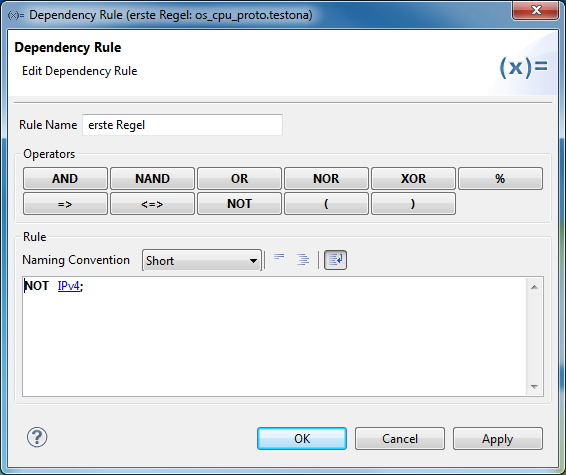
\includegraphics[scale=0.5]{dependency_rules_2.png}
  		  \caption{Abhängigkeitsregeln Bearbeitung}
     \label{ttn.depencyRulesEdit}
  \end{center}
\end{figure}

Boolesche Operatoren:\\

\begin{tabular}{ll}
AND &: Konjunktion\\
NAND &: negierte Konjunktion\\
OR &: Disjunktion\\
NOR &: negierte Disjunktion\\
XOR &: ausschließende Disjunktion\\
\% &: \glqq don't care\grqq~ Operator\\
=> &: vom A folgt B\\
<=> &: A ist gleichwertig wie B\\
NOT &: Negation\\
\end{tabular}


Durch die Verwendung dieser Operatoren wurde folgende Abhängigkeitsregel definiert:

\begin{figure}[h]
  \begin{center}
    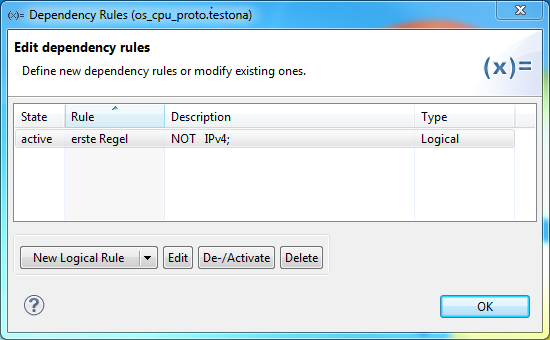
\includegraphics[scale=0.5]{dependency_rules.png}
  		  \caption{Abhängigkeitsregeln Übersicht}
     \label{ttn.depencyRules}
  \end{center}
\end{figure}

Nehmen wir die Regeln wahr, so will der Tester die Klasse \glqq IPv4\grqq~ für diese Tests nicht betrachten. Also werden nur Testfälle erzeugt, in denen dieser Parameter nicht vorkommt.


\begin{figure}[h]
  \begin{center}
    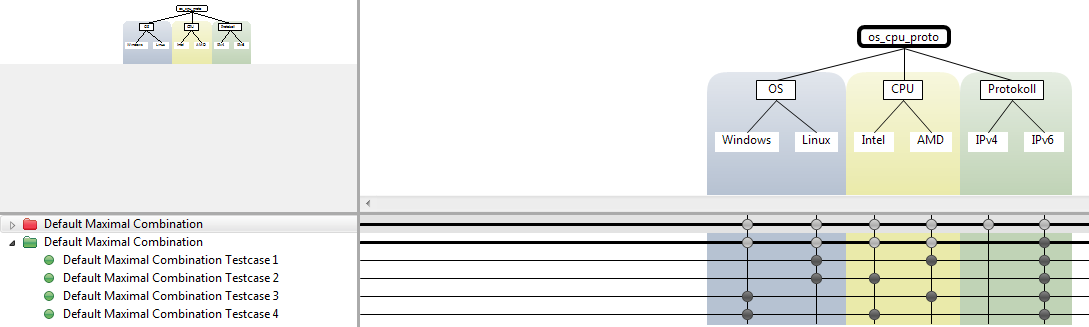
\includegraphics[scale=0.5]{dependency_rules_noParam.png}
  		  \caption{Testfälle mit Anwendung der Abhängigkeitsregeln aus \ref{ttn.depencyRulesEdit} und \ref{ttn.depencyRules}}
     \label{ttn.testsequence}
  \end{center}
\end{figure}

In diesem einfachen Beispiel wird nur ein Parameter ausgeschlossen, aber durch die Abhängigkeitsregeln kann der Tester durchaus komplexere Fälle einleiten. Betrachten wir folgendes Szenario: Ein Licht wird mit einer 5V Spannung durch eine Batterie versorgt. Die Spannung der Batterie befindet sich momentan im niedrigen Bereich. Das System hat zwei Lichtschaltern um das Licht zu steuern. Es soll die Reaktion des Systems getestet werden, wenn eins der beiden Lichtschaltern betätigt wird. Um so ein Fall zu prüfen, werden zwei verschiedene Regeln angelegt:

\begin{enumerate}
\item \textit{Lichtschalter1 XOR Lichtschalter2}
\item \textit{Spannung NOT 5V}
\end{enumerate}

Die erste Regel besagt, dass mindestens einer der beiden Lichtschalter betätigt werden muss, um das Licht einzuschalten. Die zweite Regel spezifiziert, dass nur der Fall betrachtet wird, wenn die Spannung der Batterie unter die 5V Grenze liegt. Daraus werden nur Testfälle erzeugt, die diese beide Kriterien erfüllen.





%#######################################################################################
%#######################################################################################
\newpage
\section{IBM Rational DOORS}\label{sec:DOORS}
\paragraph{}

Quality Systems \& Software (QSS) hat Anfang der 90er Jahre DOORS (Dynamic Object Oriented Requirements System) entwickelt. Die Firma Telelogic kaufte im Jahr 2000 QSS, die wiederum 2008 von IBM übernommen wurde. DOORS ist eine Anforderungsmanagement Software und ermöglicht die Verwaltung und strukturierte Aufzeichnung von Anforderungen (als Objekte). Durch eine tabellarische Ansicht der Anforderungen können die Anforderungen und die zugehörige Eingenschaften abgelesen werden. Als Eingenschaften sind eine eindeutige Identifikationsnummer, sowie vom Benutzer ausgewählte Attribute.\\


\begin{figure}[h]
  \begin{center}
    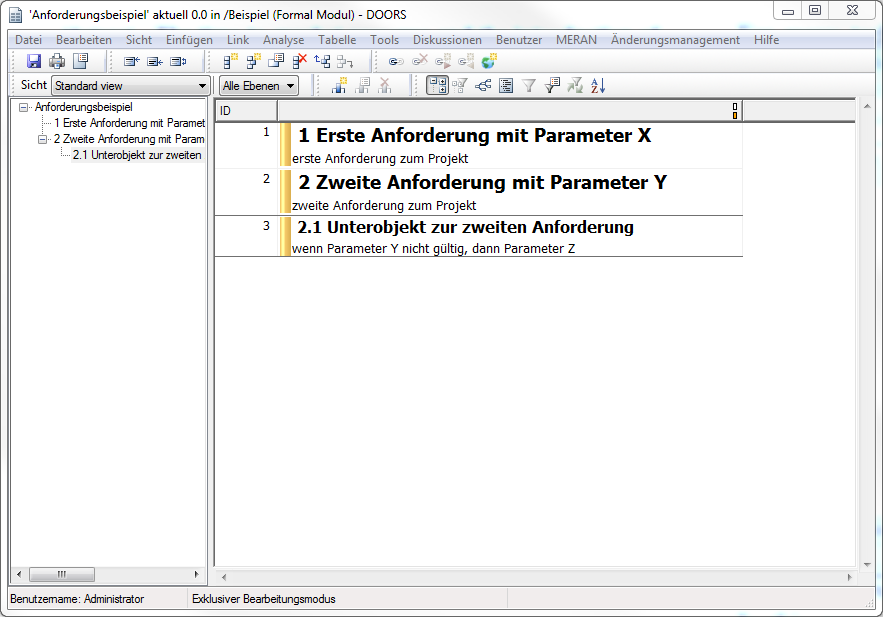
\includegraphics[scale=0.5]{doorsTable.png}
  		  \caption{Beispiel einer Tabelle in DOORS}
     \label{doors.bespiel}
  \end{center}
\end{figure}


In DOORS wird eine Tabelle \glqq Modul\grqq~ genannt. Jede Zeile innerhalb eines Moduls  ist ein Objekt und die Spalten für jedes Objekt bezeichnet man als Attribut. Ein Objekt kann Unterobjekte besitzen, indem Alternativen und weitere Anforderungen beschrieben werden (siehe Abbildung \ref{doors.bespiel}).


Um Anforderungen im Laufe des Projektes zu verfolgen (Tracing), können Anforderungen miteinander verlinkt werden. DOORS basiert sich auf eine Client - Server Anwendung mit einer proprietären Datenbank. \\


Es werden auch Schnittstellen für den Datenaustausch zur Verfügung gestellt (Testmanagement -, Modellierungs - und Changemanagementwerkzeuge) dank der Unterstützung von RIF (Requirements Interchange Format). Durch die Skriptsprache \glqq DXL\grqq~ (DOORS eXtention Language) erhält TESTONA Zugriff auf die gespeicherten Module in DOORS. \cite{Doors} \cite{Anforderungsmanagement}\\

TESTONA besitzt Klassen die DXL-Scripte ausführen, damit der Entwickler einfach und sicher Daten in DOORS abrufen kann.


%#######################################################################################
%#######################################################################################
\newpage
\section{Variantenmanagement}\label{sec:VarManag}
\paragraph{}

Variantenmanagement, wie das Wort schon verrät, behandelt verschiedene Varianten eines Produktes. Um eine Variante besser zu definieren, betrachten wir folgendes Beispiel: ein Auto \glqq A\grqq~ soll in verschiedenen Modellen gebaut werden: Kombi, Limousine und Cabrio. Alle Modellen von \glqq A\grqq~ haben die Eigenschaften eines Wagens (4 Räder, Personenkraftwagen, Türen, etc), aber sie unterscheiden sich untereinander durch die Anzahl der Passagiere oder der Größe des Wagens. Daher kann jedes gebaute Modell von \glqq A\grqq~ als eine Variante betrachtet werden.\\


Anhand des Beispieles wird klar, dass durch die steigenden Produktkomplexität bzw. -vielfalt die Identifikationsmerkmale zur Definition einer Produktvariante immer schwieriger zu vereinbaren sind. Für diese Masterarbeit ist eher wichtig, Identifikationsmerkmale zu definieren, die dazu führen, dass die Tests oder der Testablauf eines Produktes geändert werden muss (mehrere Testfälle sind nötig, neue Parameterwerte). Das heißt, wenn ein Auto als Kombi gebaut wird und danach als Cabrio angeboten wird, müssen (unter anderem) die ganze Dachfunktionen geprüft werden. Das führt dazu neue Testspezifikationen, Testabläufe und Testfälle zu erstellen, die die Funktionalität des Daches überprüfen.\\


Varianten werden oft mit Features verwechselt. Der Unterschied zwischen ein Feature und einer Variante ist sehr fein und oft abhängig vom Betrachtungspunkt. Um dem Unterschied deutlicher zu machen, werden Änderung in der Funktionalität oder Konstruktion des Autos als einer Variante betrachtet. So sollte man die Karosseriefarbe als ein Feature betrachten, weil theoretisch eine Änderung der Farbe keine Änderung in der Funktionalität oder sich auf die Leistung des Autos auswirkt (somit werden die Tests oder Testabläufe nicht beeinflusst). Ein Auto mit verschiedener Lackierung des selben Modells erzeugt keine Änderung im Testaufwand.\cite{VarMan2}\\


\begin{figure}[h]
  \begin{center}
    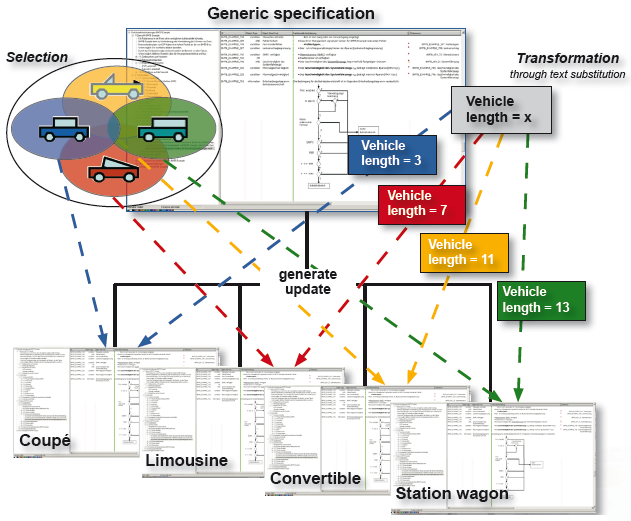
\includegraphics[scale=0.4]{varianten.png}
  		  \caption{Betrachtung von Varianten eines Wagens von der generischen Testspezifikation zur variantenspezifische Testspezifikation aus \cite{VarMan1}}
     \label{variantsOverview}
  \end{center}
\end{figure}


Das Variantenmanagement wird im Allgemeinen dazu benutzt um bei komplexere Produkte einen besseren Überblick zu haben. Hinsichtlich das Testen, können Änderung des Produktes besser erkannt werden. Somit werden die Testfälle und Testabläufe an der jeweiligen Variante angepasst. Die Abbbildung \ref{variantsOverview} betrachtet die Länge jedes Modell und erstellt aus die generische Spezifikation einzelnen Spezifikationen für jede Variante. Die Testfälle werden mit den richtigen Werten erstellt und eine bessere Testabdeckung kann gewährleistet werden.\\


In TESTONA werden  die in DOORS definierten Produktvarianten importiert. Baumelement werden an der jeweiligen Variante hinzugefügt. Wenn der Benutzer eine Variante auswählt, werden nur die in dieser Variante gültige Baumelemente angezeigt. So wird die Übersicht verbessert und der Tester kann Testfälle genauer erstellen.




%#######################################################################################
%#######################################################################################
\newpage
\section{Entwicklungsumgebung und Programmiersprache}
\paragraph{}
TESTONA wurde ursprünglich in der Programmiersprache \glqq Pascal\grqq entwickelt. Mit der Weiterentwicklung wurde das Programm an \glqq C\grqq portiert. Durch den Kauf von Berner \& Mattner in 2008 wurde TESTONA bis zum jetzigen Zeitpunkt auf Java übersetzt und wird seit 2010 mit der Entwicklungsumgebung Eclipse entwickelt.

%#######################################################################################
\subsection{Eclipse}
\paragraph{}
Eclipse ist der Nachfolger von \glqq IMB Visual Age for Java\grqq~ und ist ein quelloffenes Programmierwerkzeug zur Entwicklung verschiedener Arten von Software. Ursprünglich wurde Eclipse als integrierte Entwicklungsumgebung für Java benutzt. Dank seiner Bedienbarkeit und Erweiterung ist Eclipse mittlerweile für die Entwicklung in verschiedenen Programmiersprachen bekannt (unter anderem C/C++ und PHP). Die am 25 Juni 2014 veröffentliche Version \glqq Luna\grqq~ (Eclipse 4.4) ist der aktuellste Stand der Software. \\

Mit Eclipse 3.0 hat sich die Grundarchitektur von Eclipse geändert. Seit diesem Zeitpunkt ist Eclipse nur ein Kern, der einzelne Plug-ins lädt. Jedes Plug-in stellt eine oder verschiedene Funktionalitäten zur Verfügung. Darauf aufbauend existiert die \glqq Rich Client Platform\grqq~ (RCP). Diese ermöglicht Entwicklern Anwendungen zu programmieren, die auf das Eclipse Framework aufbauen, aber unabhängig von der Eclipse IDE ist\cite{EclipseRCP} \cite{Eclipse}. Dies ist einer der Hauptgründe warum TESTONA zu Java und Eclipse migriert wurde. Durch RCP können verschiedene Programmversionen (Light, Express, Professional, Enterprise) besser verwaltet werden. Durch die RCP Architektur werden auch verschiedene Funktionalitäten voneinander getrennt. Das hilft bei der Weiterentwicklung sowie bei der Pflege des Programms, da mehrere Entwickler gleichzeitig an verschiedenen Plug-ins arbeiten können. Der Aufwand wird niedrig gehalten, weil nur ein Workspace genutzt wird. Bei der Erstellung von verschiedene Versionen werden nur die Plug-ins geladen, die nötig sind.


%#######################################################################################
\subsection{Plug-ins}
\paragraph{}
Ein Plug-in ist die kleinste ausführbare Softwarekomponente für Eclipse. Um eine Anwendung mit Eclipse RCP zu schreiben, werden mindestens diese drei Plug-ins benötigt:

\begin{itemize}
\item Eclipse Core Plattform: steuert den Lebenszyklus der Eclipse Anwendung
\item Stardard Widget Toolkit: Programmierbibliothek zur Erstellung von grafischen Oberflächen
\item JFace: User Interface Toolkit für komplexere Widgets
\end{itemize}

Weitere Plug-Ins, von der Eclipse Foundation implementiert, stehen den Programmierern zur Verfügung und unter \textit{marketplace.eclipse.org} können auch von Privatentwicklern programmierte Plug-Ins heruntergeladen werden. \cite{Eclipse}\\

Plug-ins beinhalten den Java-Code der, wie gewöhnlich, in verschiedene Pakete und Klassen strukturiert werden kann. Sinnvoll ist, dass jedes Plug-in eine Funktionalität des gesamten Programms repräsentiert, wie zum Beispiel, Variantenmanagement oder Autosave.\\

Testona besteht momentan aus viele verschiedene Plug-ins, wobei jedes Plug-in eine bestimmte Funktion oder Feature des Programms implementiert. Zum Beispiel gibt es für jede Version (Light, Express, Professional und Enterprise) von TESTONA ein Plug-in indem die nötige Plug-ins für die gewünschte Version geladen werden.\\

Ein Plug-in besteht in der Regel aus folgenden Einheiten:

\begin{itemize}
\item \textbf{JRE System Library:} beinhaltet alle Systembibliotheken von der Java Runtime Enviroment, dass der jeweilige Plug-in benötigt
\item \textbf{Plug-in Dependencies:} schließt die Abhängigkeiten des Plug-ins mit der Eclipse Umgebung und anderen implementierten Plug-ins ein
\item \textbf{src:} bezieht die Pakete und Java-Klassen ein
\item \textbf{icons:} hier befinden sich die Bilderdateien (.gif, .png, etc) die in den Klassen für die Benutzeroberfläche  aufgerufen werden
\item \textbf{META-INF:} gibt eine Übersicht aller Einstellungen des Plug-ins, sowie die Möglichkeit diese über eine graphische Oberfläche zu bearbeiten
\item \textbf{build.properties:} beinhalten die Einstellungen für das Compilieren des Plug-in. Es kann auch über die META-INF Datei bearbeitet werden.
\item \textbf{plugin.xml:} hier werden die nötigen Erweiterungen für das Plug-in definiert. Es ist möglich direkt die \textit{xml} Datei zu bearbeiten, oder die META-INF Oberfläche benutzen.
\end{itemize}

Ein Plug-in kann durchaus mehrere Einheiten oder Elemente beinhalten, wie zum Beispiel weitere \textit{resource} Ordner oder ein Dokumentationsordner mit wichtigen Dokumenten zum Plug-in.




%#######################################################################################
\subsection{Standard Widget Toolkit (SWT)}
\paragraph{}
SWT ist eine IBM Programmierbibliothek (seit 2001) für die Programmierung grafischen Oberflächen unter Java. Die Bibliothek benutzt, im Gegensatz zu Swing\footnote{Programmierschnittstelle und Grafikbibliothek für Java zum programmieren von grafischen Benutzeroberflächen.}, die nativen grafischen Elemente des jeweiligen Betriebssystems und ermöglicht die Erstellung von Anwendungen, die optisch ähnlich wie die nativen Anwendungen des Betriebssystems aussehen. Durch die Verwendung der nativen grafischen Elemente, kann das Toolkit sofort Änderungen in das \glqq look and feel\grqq~ des Betriebssystems in der Anwendung aktualisieren und beinhaltet ein konstantes Programmiermodel in alle Plattformen.
\cite{EclipseSWT}\\

SWT beinhaltet sehr viele komplexe Eigenschaften. Aber für eine robuste und benutzbare Anwendung zur Programmieren sind nur die Grundkenntnisse nötig. Eine typische SWT Anwendung hat folgende Struktur:

\begin{itemize}
\item Ein \textit{Display} deklarieren (repräsentiert die SWT Modus)
\item Erstellen eines \textit{Shell}, welche als Hauptfenster dient
\item Erzeugung eines Widgets
\item Initialisierung der Widgetsparameter
\item Öffnen des Fensters
\item Starten der Event-Schleife bis eine Abbruchbedingung erfüllt wird (Schließen des Fenster vom Benutzer)
\item Entsorgen des Displays
\end{itemize}

\begin{lstlisting}[caption={Beispiel einer SWT Anwendung}, captionpos=b]
   public static void main (String[] args) {
      Display display = new Display();
      Shell shell = new Shell(display);
      Label label = new Label(shell, SWT.CENTER);
      label.setText("Hello_world");
      label.setBounds(shell.getClientArea());
      shell.open();
      while (!shell.isDisposed()) {
         if (!display.readAndDispatch())
         		display.sleep();
      }
      display.dispose();
   }
\end{lstlisting}


SWT wird in TESTONA eingesetzt, damit das Aussehen der Benutzeroberfläche automatisch aktualisiert an des jeweilige Betriebssystem angepasst wird. Es erspart auch sehr viel Entwicklungszeit, da die Grafikkomponenten des Programms nicht für jedes Betriebssystem programmiert werden müssen.





%#######################################################################################
\subsection{JFace}
\paragraph{}
JFace ist ein User Interface Toolkit, das auf die von SWT gelieferten Basiskomponenten setzt und stellt die Abstraktionsschicht für den Zugriff auf die Komponenten bereit. Es beinhaltet Klassen zur Handhabung gemeinsame Programmieraufgaben, wie zum Beispiel:


\begin{itemize}
\item Viewers: Verbindung von Oberflächenelementen zum Datenmodell
\item Actions: definiert Benutzeraktionen und spezifiziert wo diese zur Verfügung stehen
\item Bilder und Fonts: gemeinsame Muster für den Umgang mit Bilder und Fonts
\item Dialoge und Wizards: Framework für komplexere Interaktionen mit dem Benutzer
\item Feldassistent: Klassen die dem Benutzer für richtige Inhaltsauswahl bei Dialogen oder Formularen Hilfe anbieten
\end{itemize}


SWT ist komplett unabhängig von JFace (und Plattform Code), aber JFace wurde konzipiert um SWT  bei allgemeinen Benutzerinteraktionen zu unterstützen. Eclipse ist wohl das bekannteste Programm das JFace benutzt.\cite{EclipseHelp}\\



%#######################################################################################
\subsection{Tags}\label{sub.Tags}
\paragraph{}

Ein \textit{Tag} ist ein Objekt, das auf EMF (Eclipse Modeling Framework) basiert. EMF ist ein Java Framework der Eclipse-Open-Source Gemeinschaft für die automatische Erzeugung von Quelltext aus Modellen \cite{EclipseRCP}.  Bei EMF wird die Problemstellung in einem Klassendiagramm beschrieben. Hier werden die Eigenschaften und Attribute der Klassen eingetragen um daraus wird der Quelltext generiert. Die Objekte können ohne großen Aufwand serialisiert und validiert werden und mögliche Fehlerquellen werden ausgeschlossen. In das Ecore-Modell werden die Klassen definiert und in Pakete eingeteilt. Der erzeugte Quelltext kann dann vom Benutzer ergänzt werden.\\



\textit{Tags} dienen hauptsächlich dazu um Eigenschaften anderer Objekte zu beschreiben. In \textit{VariantsTag} werden zum Beispiel  Varianten gespeichert. Wenn in einem Projekt verschiedene Varianten zur Verfügung stehen, wird es dazu kommen, dass ein Baumelement nicht in allen Varianten auftritt. Das Baumelement wird ein \textit{VariantsTag} besitzen, das spezifiziert zur welchen Varianten das Baumelement gehört. in \textit{RequirementTags} werden die Anforderungen gespeichert die an einem Baumelement verknüpft worden sind. Für die farbige Trennung zwischen Knotenpunkten im Klassifikationsbaumeditor ist ein \textit{ColoringTag} zuständig.\\

Die Grundstruktur eines \textit{Tags} besteht aus:

\begin{itemize}
\item Name
\item Identifikationsnummer
\item Typ
\item Inhalt
\item Zugriffsrechte
\end{itemize}


Je nach Zweck können die Klassen um weitere Attribute erweitert werden. Durch die Vererbung und Quelltextgenerierung wird sichergestellt, dass alle \textit{Tags} innerhalb TESTONA kompatibel sind. Anhand der Serialisierung können die \textit{Tags} in die TESTONA Datei im XML-Format gespeichert werden und auch ausgelesen werden. Um Parameter in Baumelementen zur speichern, wird auf diesem Modell aufgebaut. Weitere Erörtungen in Kapitel \ref{sec.parameterspeicherung} und \ref{sub.ParameterTag} .
\chapter{Lösungsansatz}\label{chp:loesungsansatz}

Um besser den Lösungsansatz zu verstehen, wird erstmal der Ablauf von der Erstellung von Anforderung bis zu einem Testfall erläutert. Als erstes wird in DOORS alle schon vordefinierte Anforderungen eingetragen (siehe \ref{sec:DOORS}). In diesen Anforderung können Parameter vorkommen, die für die Testfälle relevant sind. Die Parameter werden als folgendes in einer Anforderung eintragen:\\

\begin{center}
\#param [\textit{Parametername}]\\
\#param [max\_Geschwindigkeit]\\
Das Auto hat eine Maximalgeschwindigkeit von \#param[max\_geschwindigkeit] km/h
\end{center}

Die Parameter sind in einer Parameter-Tabelle definiert, wo die jeweilige Parameterwerte eingetragen werden. Der Grund, dass es eine extra Tabelle für Parameter gibt, kommt daher, dass die Parameter in der Regel pro Variante verschiedene Werte annehmen. Zum Beispiel beträgt die maximale Geschwindigkeit bei einem Cabrio 100 km/h  und bei einem Kombi 150 km/h. Dank dieser Tabelle werden die Varianten (Cabrio und Kombi) die richtige Parameterwerte zugewiesen.\\

Da Parameterwerte und Varianten schon verlinkt sind, müssen die Anforderungen, die Parametern beinhalten, mit der Parametertabelle manuell verlinkt werden. Wenn dieser Vorgang abgeschlossen ist, kann über die TESTONA Oberfläche die Verbindung zu DOORS aufgebaut werden um die nötigen Informationen zu importieren. Es wird davon ausgegangen, dass der Tester bereits ein Klassifikationsbaum passend zum testenden Produkt und die dazu gehörige Anforderungen erstellt hat. Jetzt können die in DOORS definierte Varianten importiert werden. Als erstes muss der Tester die Baumelemente der richtigen Variante zuordnen (durch ein Ausschlussverfahren, es wird angenommen, dass alle Baumelemente in alle Varianten gültig sind). 


%#######################################################################################
%#######################################################################################
\newpage
\section{Parameterspeicherung}\label{sec.parameterspeicherung}
\paragraph{}
 
Um die Parameter erfolgreich in TESTONA zu speichern, müssen diese aus DOORS importiert werden und aus den Anforderungen gelesen werden. Durch eine gezielte Anfrage an DOORS, über eine Java API, kann die Parametertabelle in TESTONA geladen werden. Die darin bestimmte Beziehungen (Parameterwert zu Variante) müssen fest in die TESTONA Datei gespeichert werden, damit diese auch ohne eine DOORS Verbindung zur Verfügung steht. Als erstes werden die Parameterwerte in Objekte gespeichert und einen \textit{Tag} (Kennzeichen) gegeben und nach Programmende in die TESTONA Datei im XML Format gespeichert. Dank des \textit{Tags} kann beim Programmstart wieder der Parameterwert gelesen werden und währen das Programm ausgeführt wird, Änderungen vornehmen.\\

Einer der Besonderheiten von TESTONA in Verbindung mit MERAN ist, dass Anforderungen and Baumelemente per Drag\&Drop verknüpft werden können. Mit dieser Funktion muss der Tester die Anforderung mit einem dazu gehörigen Baumelement verknüpfen (auslösendes Ereignis der Parameterspeicherung). Damit das Programm die Aktion des Benutzer mitbekommt, wird an dieser Stelle ein \textit{Listener} implementiert. Der \textit{Listener} bekommt verschiedene Nachrichten von Ereignisse die gefiltert werden müssen. Wenn die Nachricht empfangen wird, dass eine Anforderung an ein Baumelement verknüpft wurde, muss eine zu programmierende Methode das Anforderungstext von dieses Baumelement lesen und nach Parameter suchen. Als erstes wird davon ausgegangen, dass ein Baumelement nur eine Anforderung beinhalten kann und eine Anforderung nur ein Parameter beinhaltet. Wird in der gelesenen Anforderung ein Parameter gefunden, so müssen die möglichen Werten dieses Parameters aus die DOORS Parametertabelle gelesen und gespeichert werden. An dieser Stelle beginnt die Parameterspeicherung.\\

Für die Parameterspeicherung ergeben sich zwei Lösungswege. Die erste Lösung lautet, die Parametertabelle beim importieren der Anforderung gleich in TESTONA zu speichern. Diese Lösung hat den Vorteil, dass später eine Verbindung zu DOORS nicht mehr notwendig ist. Somit muss während der Parametersuche nach eine Verbindung mit DOORS nicht geprüft werden, oder die Verbindung muss nicht wieder aufgebaut werden. Das heißt der Benutzer muss sich nur einmal mit DOORS Verbinden und kann in der Zukunft problemlos die Anforderungen an Baumelement verlinken und zugleich werden die Parameter gelesen und gespeichert. Der Nachteil ist, dass möglicherweise unnötige Daten in TESTONA gespeichert werden.\\

Die zweite Lösung ist der Gegensatz zu die erste. Hier werden jeweils nur die Daten gespeichert, die der Benutzer im Moment verbraucht. Wird eine Anforderung an einem Baumelement verlinkt, so muss eine Verbindung zu DOORS aufgebaut werden (wenn sie nicht vorhanden ist) und die Parametertabelle aufrufen und in TESTONA speichern. Der große Nachteil dieser Lösung ist, dass der Benutzer möglicherweise nicht eine Verbindung zu DOORS aufbauen kann (Server nicht Vorhanden, keine Zugriff Möglichkeiten, etc.). Welcher der beiden Lösungen implementiert wird, wird erst genauer analysiert und ist auch abhängig von den Anforderungen verschiedener Kunden und wie diese TESTONA anwenden. Die implementierte Lösung wird in Kapitel \ref{chp:systementwurf} vorgestellt und begründet.\\


Sind die Parameterwerte in TESTONA vorhanden, müssen diese an der richtigen Variante noch zugeordnet werden. Dafür ist vorgesehen, dass der Parameterwert als Eigenschaft des Baumelementes gespeichert wird (als ein \textit{Tag} Objekt). Die Darstellungsstruktur für die Variantenansicht ist etwa folgendermaßen definiert:\\

\begin{figure}[h!]
  \begin{center}
    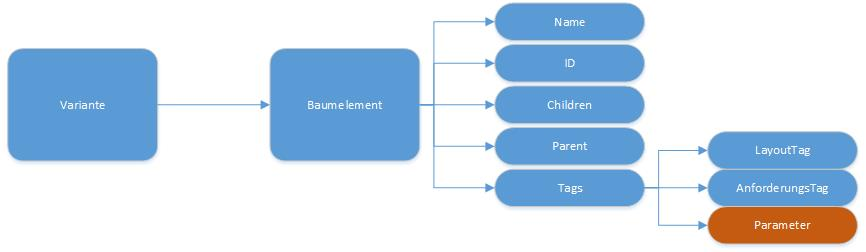
\includegraphics[scale=0.5]{4_1_UML_Var_TreeItem_Properties.jpg}
  		  \caption{Darstellung der TESTONA Objekte für die Parameterspeicherung}
     \label{ttn.objectGraph}
  \end{center}
\end{figure}


Somit kann jetzt in TESTONA ein Parameterwert mit einer Variante und ein Baumelement verknüpft werden. Als Ergebnis werden folgenden Beziehungen erwartet:

\begin{center}
\textbf{Anforderung 1: }Das Auto hat eine Maximalgeschwindigkeit von \#param[max\_Geschwindigkeit] km/h.
\end{center}

\begin{table}[h]
\begin{center}
	\begin{tabular}{|l||c|c|}
	 \hline
	 Variante &Maximalgeschwindigkeit &Anforderung\\
	 \hline\hline
	 Cabrio   &100                      & 1\\
	 \hline
	 Kombi    &150                      & 1\\
	 \hline
	 Limo     &250                      & 1\\
	 \hline
	\end{tabular}
	
	\caption{Beispiel für die Zuordnung zwischen Varianten und Parameterwert aus einer Anforderung}
	\label{table:4TestCases}
\end{center}
\end{table}

Wenn ein Baumelement mehr als eine Anforderung beinhaltet, mit verschiedene Parametern, wird die aktive Variante entscheiden, welches Parameter ausgewertet wird. Dabei muss beachtet werden, dass vorhandene Parameterwerte und Anforderung nicht gelöscht oder überschrieben werden. Wichtig ist auch, das ein Baumelement verschiedene Parameter repräsentieren kann. Für die Darstellung wird die aktive Variante entscheiden, welches Parameter angesprochen wird, sowie was für ein Parameterwert.\\

\begin{figure}[h!]
  \begin{center}
    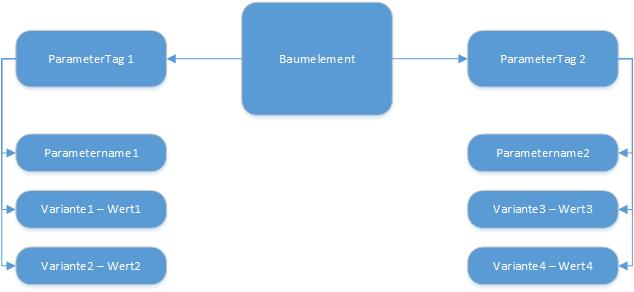
\includegraphics[scale=0.7]{4_1_UML_TreeItem_ParameterTags.jpg}
  		  \caption{Darstellung eines Baumelementes mit zwei verschiedene Parametern und vier Varianten}
     \label{ttn.treeitem_vars}
  \end{center}
\end{figure}

%#######################################################################################
%#######################################################################################
\newpage
\section{Visualisierung}\label{sec.visialisierung}
\paragraph{}
%1.2 Wenn der Tester die Ansicht zwischen Varianten ändert, muss der Wert hinter dem Parameter auf die jeweilige Variante aktualisiert werden (maximale Geschwindigkeit von Cabrio = x, Limo = y, Kombi = z).

% Als Ergebnis soll bei der Änderung der Variantenansicht, auch  geändert werden. Ist die Variante \textit{Cabrio} aktiv, so muss das Baumelement mit die maximalen Türanzahl der Wert zwei anzeigen. Wird die Variantenansicht geändert auf die Variante \textit{Kombi}, so muss das Baumelement der Wert fünf anzeigen.

Wenn die Beziehungen zwischen Varianten, Parameter und Anforderungen erfolgreich entstanden sind, können jetzt die gespeicherte Parameterwerte angezeigt werden. Hier ist gefordert, dass wenn der Benutzer die Variantenansicht ändert (durch Betätigung an der Benutzeroberfläche) die Beschriftung (\textit{Label}) des Baumelements (Maximalgeschwindigkeit von Generic = X, Cabrio = 150, Kombi = 200) aktualisiert werden.\\



\begin{figure}[h!]
  \begin{center}
    
\includegraphics{4_2_Change_Var_Generic.png}
    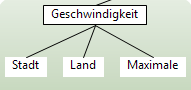
\includegraphics[scale=0.8]{4_2_Change_Var_Generic_Tree.png}
  		  \caption{Aktive Variante Generic (default)}
     \label{ttn.generic}
  \end{center}
\end{figure}

\begin{figure}[h!]
  \begin{center}
    
\includegraphics{4_2_Change_Var_Cabrio.png}
    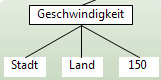
\includegraphics[scale=0.9]{4_2_Change_Var_Cabrio_Tree.png}
  		  \caption{Aktive Variante Cabrio}
     \label{ttn.2}
  \end{center}
\end{figure}

\begin{figure}[h!]
  \begin{center}
    
\includegraphics{4_2_Change_Var_Kombi.png}
    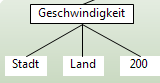
\includegraphics[scale=0.9]{4_2_Change_Var_Kombi_Tree.png}
  		  \caption{Aktive Variante Kombi}
     \label{ttn.3}
  \end{center}
\end{figure}

Dafür muss ein \textit{Listener} beim Ändern der Ansicht eine Methode aufrufen, die sich um das aktualisieren der Werte und Neuzeichnung. Die Werten werden dynamisch aus den Inhalten der Baumelemente gelesen. Zur Erinnerung die Werte sind als \textit{Tag} im jeden Baumelement gespeichert (siehe Abbildungen \ref{ttn.objectGraph} und \ref{ttn.treeitem_vars})


%#######################################################################################
%#######################################################################################
\newpage
\section{Testgültigkeit}
\paragraph{}
%Innerhalb einer Variante auf Testfallduplikate überprüfen anhand der Paramerterwerte
%Testfallabdeckung + Prozessoptmierung
Wenn TESTONA in der Lage ist, die Parameterwerte abhängig von der Variante darzustellen, soll möglicherweise nach duplizierte Testfälle gesucht werden. Es kann dazu kommen, dass ein Testfall sich dupliziert, da zwei oder mehrere Parameter den gleichen Wert besitzen.Folgendes einfaches Beispiel:\\

\begin{figure}[h!]
  \begin{center}
    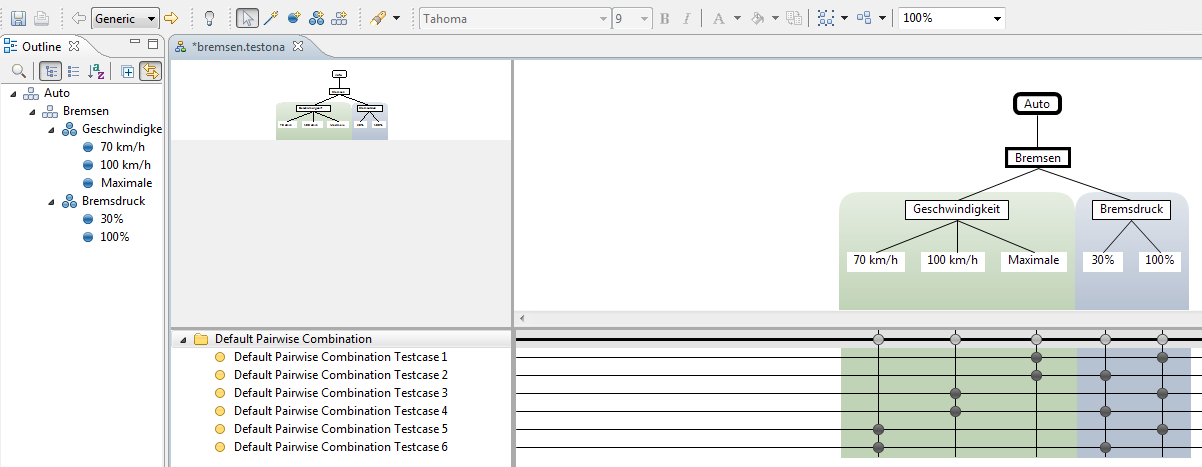
\includegraphics[scale=0.4]{4_3_generic.png}
  		  \caption{Das generische Baum}
     \label{ttn.cases_generic}
  \end{center}
\end{figure}

\begin{figure}[h!]
  \begin{center}
    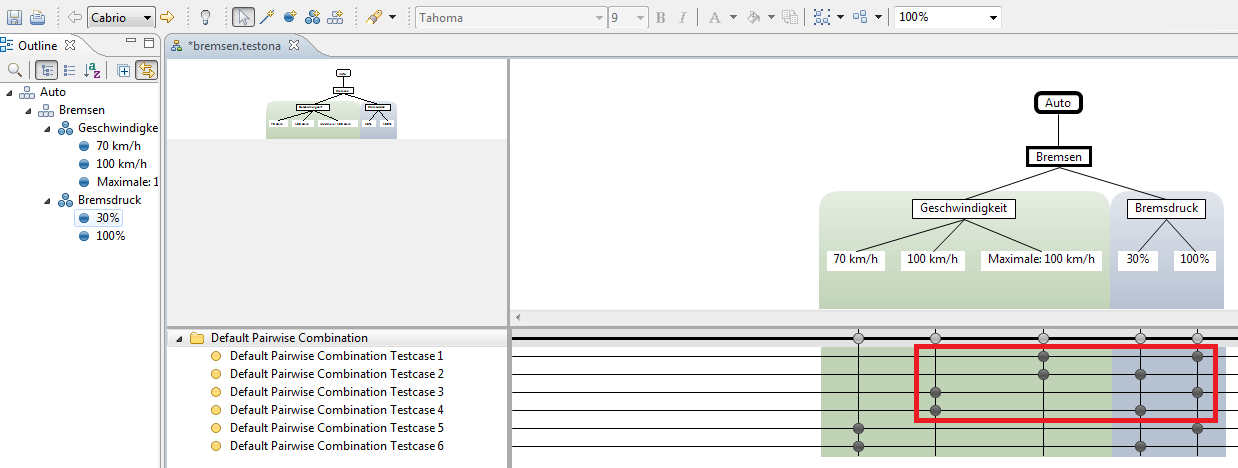
\includegraphics[scale=0.4]{4_3_cabrio.png}
  		  \caption{Aktive Variante Cabrio}
     \label{ttn.cases_cabrio}
  \end{center}
\end{figure}

\begin{figure}[h!]
  \begin{center}
    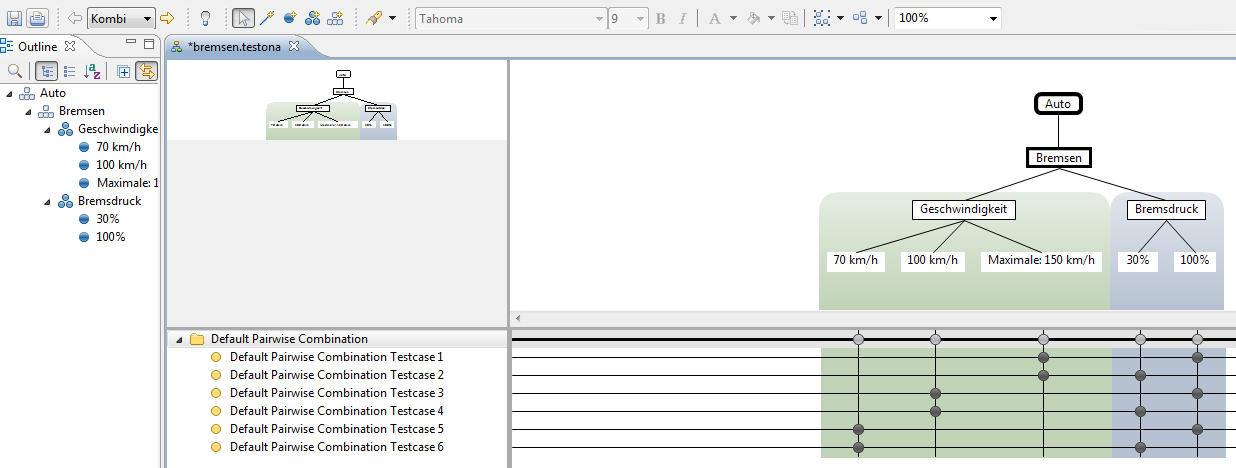
\includegraphics[scale=0.4]{4_3_kombi.png}
  		  \caption{Aktive Variante Kombi}
     \label{ttn.cases_kombi}
  \end{center}
\end{figure}

Es ist leicht zu erkennen, dass die Testfälle eins bis vier in der Variante \glqq Cabrio\grqq~ dupliziert sind. Bei so ein minimalistisches Baum sind solche Fälle einfach zu erkennen. Bei einen komplexeren Baum mit sehr viele Klassen kann es schnell zur Unübersichtlichkeit kommen und duplizierte Testfälle werden übersehen oder nicht erkannt.\\

Hier muss bei der Testfallgenerierung zusätzlich geachtet werden (vorausgesetzt es gibt Varianten und Parameterwerte), dass nicht nur die Baumelemente betrachtet werden, sondern auch die Parameterwerte.\\

Dafür müssen alle Klassen (Endknoten) unterhalb der gleichen Klassifikation überprüft werden. Nach das obenstehende Beispiel, müssen die Klassen \glqq 70 km/h\grqq , \glqq 100 km/h\grqq~ und \glqq Maximale\grqq~ verglichen werden. Da \glqq Maximale\grqq~ bei jeder Variante ein anderen Wert annimmt, muss hier überprüft werden, das bei jeder Variante, sich der Wert nicht wiederholt. Die Werte werden aus den geplanten \textit{ParameterTag} (siehe Abbildung \ref{ttn.objectGraph}) gelesen.

%#######################################################################################
%#######################################################################################
\newpage
\section{Optimierungskriterien}
\paragraph{}
%Testablauf optimieren in Betrachtung auf nur gültige Baumelemente in einer Variante und mögliche Testduplikate,

%#######################################################################################
%#######################################################################################
\newpage
\section{Benutzeroberfläche}
\paragraph{}

%Um die Handhabung der Varianten bezogen auf die Testfälle und die Testgenerierung benutzerfreundlicher und effizienter zu gestalten, soll die Benutzung des Variantenmanagements durch einen Testingenieur untersucht werden. Resultierend aus den erworbenen Erkenntnissen wird das Lösungsdesign für eine Erweiterung des bestehenden Variantenmanagements in TESTONA konzipiert.

%nach besprechen mit kollegen keine änderung nötig erstmal \\

Eine Änderung der Benutzeroberfläche von TESTONA wurde mit Kollegen in der Entwicklung offen diskutiert. Als Ergebnis konnten wir (aus Sicht der Entwickler) feststellen, dass die bisherige Lösung als gut und intuitiv zu Bezeichnen ist.\\

Um weitere Meinungen und Lösungsvorschläge zu sammeln habe ich Testingenieure innerhalb Berner \& Mattner die TESTONA mit Kunden anwenden befragt. Dabei stellte sich bei einem Ingenieur heraus, dass die Aktivierung der Variantenansicht als extra Schritt als \glqq unnötig\grqq~ bezeichnet wurde. Es wurde gewünscht, dass die Variantenansicht als Hauptansicht definiert wird. Das es ein Unterschied zwischen beiden Ansichten gibt liegt daran, dass es verschiedene Etappen repräsentieren. Die Hauptansicht bietet verschiedene Features die in der Variantenansicht mit Variantenmanagement Features ergänzt werden. Dabei wird noch begründet, dass die Trennung zur Übersicht sehr viel beitragt.\\

Als Ergebnis wurde festgelegt, dass für in dieser Arbeit gestellte Problemfrage nicht zur Unübersichtlichkeit der Benutzeroberfläche beiträgt. Es wird erhofft, außer die Erweiterung der Funktionalität, dass auch die Übersicht dabei verbessert wird. Die Trennung zwischen die Hauptansicht und die Variantenansicht wird behalten sowie die Lösung der Pfeile und Drop-Down Menü (siebe Abbildungen \ref{ttn.generic}, \ref{ttn.2}, \ref{ttn.3}).

\chapter{Systementwurf}\label{chp:systementwurf}


%#######################################################################################
%#######################################################################################
\section{Variantenmanagement und Parameter}
\paragraph{}

Die Lösung zum Speichern und Darstellen der Parameterwerte abhängig der aktiven Variante wird im diesem Kapitel erläutert.\\

\begin{figure}[h!]
  \begin{center}
    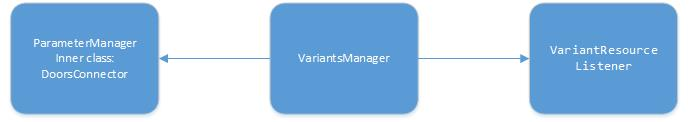
\includegraphics[scale=0.7]{5_1_klassenuebersicht.jpg}
  		  \caption{Einfache Übersicht der Klassen}
     \label{ttn.verbindung.klassen.loesung}
  \end{center}
\end{figure}


Um eine genauere Darstellung aller Klassen, bitte siehe Anhang \ref{A.PM.Diagramm}. Der Ablauf für das Speichern eines Parameters in einem Baumelement sieht folgendermaßen aus:
\begin{enumerate}
\item Benutzer verknüpft eine Anforderung an einem Baumelement
\item Der \textit{Listener} meldet das eine Änderung vorgenommen wird und gibt die Informationen weiter
\item Der \textit{VariantsManager} lädt und übergibt die nötige Informationen an das \textit{ParameterManager}
\item Der \textit{ParameterManager} lädt, sucht und erstellt ein \textit{ParameterTag}  und gibt das Befehl, dass ein \textit{ParameterTag} an ein Baumelement hinzugefügt werden muss.
\item Der \textit{ParameterManager} gibt das Befehl an das \textit{Listener} weiter
\item Das Befehl wird an die Befehlskette angehängt
\end{enumerate}

In den nächsten Unterkapiteln wird die Aufgaben der jeweiligen Klassen erläutert und der Ablauf ausführlicher erklärt.


%#######################################################################################
\subsection{VariantsManager}\label{sub.VariantsManager}
Die Hauptaufgabe des \textit{VariantsManager} ist die Varianten zu Zuordnen. Hier werden Baumelemente zu Varianten hinzugefügt und gelöscht. Dabei muss das Klassifikationsbaum neu gezeichnet werden. Diese Klasse kümmert sich auch, um die Umschaltung zwischen Varianten in der Variantenansicht (siehe Abbildung \ref{ttn.generic}) und die Richtige Darstellung der Baumelemente mit aktuelle Informationen.\\


Für die  Zwecke dieser Arbeit, wurde diese Klasse erweitert. Um die Aufgaben dieser Klasse zu erläutern, wird der Vorgang des Hinzufügen eines Parameters an einem Baumelement dargestellt. Der \textit{VariantsManager} setzt die Baumelement - ID und die Anforderungskennung in der Klasse \textit{ParameterManager}. Die Klasse dient als Schnittstelle zwischen der \textit{Listener} (siehe Kapitel \ref{sub:RSListner}) und die Klasse \textit{ParameterManager}  (siehe Kapitel \ref{sub:ParameterManager}).\\


Die Aufgabe des \textit{Listeners} lautet, dem \textit{VariantsManager} zu melden, wenn Änderung\footnote{Aktionen werden vom Benutzer ausgelöst anhand von Bedienelemente in der Benutzeroberfläche} geschehen werden oder geschehen sind. Im \textit{Listener} werden die benötigte Informationen gefiltert und an dieser Klasse weitergegeben, damit Änderung vorgenommen werden können. Im Fall der Parameterersetzung sind es die Identifikationsnummer eines Baumelementes und die Anforderungskennung der verlinkte Anforderung. Diese beide Kennungen diesen dazu, dass der \textit{VariantsManager} die jeweiligen Objekte (ein Baumelement und eine Anforderung) laden kann. Diese Objekte werden dann an der Klasse \textit{ParameterManager} übergeben.\\


Das angesprochene Baumelement muss aus das TESTONA-Diagramm geladen werden. Anhand der Identifikationsnummer werden die verschiedene Baumelemente einzeln abgefragt bis das richtige Baumelement gefunden wurde. Danach wird das Baumelement an das ParameterManager Objekt übergeben.\\


Im Fall von der Anforderungskennung, werden mehrere Informationen übergeben. Die Anforderungskennung wird in einer lokalen Variable vom ParameterManager Objekt gespeichert. Damit der Inhalt der Anforderung gelesen werden kann, müssen alle in TESTONA gespeicherte Anforderung an das ParameterManager-Objekt übergeben werden. Die gespeicherten \textit{Tags} in das TESTONA Objekt werden abfragt um folgende Objekte an das ParameterManager Objekt zu übergeben:


\begin{itemize}
\item \textbf{RequirementsConnetionTag}: beinhaltet die Information zur Datenbankverbindung, unter anderem die Verbindungsidentifikation (DOORS), das Modul(Tabelle) wo die Anforderung gespeichert ist und die Schnittstelle zur Datenbank. Anhand dieser Informationen wird die Verbindung zur Datenbank später aufgebaut.
\item \textbf{RequirementsListTag}: ist eine \textit{Map} mit alle in TESTONA gespeicherten Anforderungen. Das \textit{Key} ist die Anforderungsidentifikationsnummer und der Wert der Inhalt der Anforderung. Eine Anforderung aus dieser Liste wurde an das Baumelement verknüpft.
\item \textbf{VariantListTag}: eine Liste mit alle in TESTONA definierten Varianten.
\end{itemize}


Anhand dieser Informationen kann die Klasse \textit{ParameterManager} ein Parameter an ein Baumelement hinzufügen. Parameter können nicht nur hinzugefügt werden, sondern aus gelöscht werden. Ein Parameter wird aus einem Baumelement gelöscht, indem die verknüpfte Anforderung vom Baumelement entfernt wird. Der Ablauft für das Löschen eines Parameter ist im Grunde der gleiche als beim hinzufügen. Zunächst werden die Funktionen des \textit{Listeners} erörtert.




%#######################################################################################
\subsection{ResourceSetListener}\label{sub:RSListner}
Das auslösendes Element ist, dass der Benutzer eine Anforderung mit einen Baumelement verknüpft. Um dieses Geschehen abzufragen muss ein \textit{Listener} programmiert werden, dass das Interface \textit{ResourceSetListener}\footnote{http://download.eclipse.org/modeling/emf/transaction/javadoc/1.0.3/org/eclipse/emf/transaction/ResourceSetListener.html} implementiert. Da dass \textit{VariantsManager} ein solcher \textit{Listener} bereits besitzt, wurde dieser erweitert. Die Aufgabe des \textit{ResourceSetListener} ist, dem Benutzer zu benachrichtigen, wenn sich eine Ressource ändert. Das \textit{Listener}  \glqq hört\grqq~ auf die reinkommenden Nachrichten (\textit{ResourceSetChangeEvent}) und wertet den Inhalt dieses Events aus.\\

Das \textit{Listener} implementiert zwei Methoden die für das Abfragen der Events relevant sind. Eine davon heißt \textit{resourceSetChanged(Event e)}. Diese Methode wird aufgerufen, wenn sich eine Ressource ändert. Am Anfang wurde diese Methode  für das Abhören von Events (wenn eine Anforderung zu einem Baumelement verknüpft wird) favorisiert um danach die Parameterersetzung zu triggern. Nach der Implementierung konnte ich feststellen, dass die Methode keine Schreibrechte auf die Baumelemente besitzt. Da die Ressource zu diesem Zeitpunkt sich schon geändert hat.\\


Um die Schreibrechte zu besitzen, wurde dann die Methode \textit{transactionAboutToCommit(Event e)} betrachtet. Diese Methode wird aufgerufen bevor eine Änderung geschieht. Es wird benachrichtigt, dass eine Änderung geschehen wird und welche Objekte (ein Baumelement und die angehängte Anforderung) betrachtet werden. Zu diesem Zeitpunkt besitzt die Klasse noch Schreibrechte auf die Baumelemente und kann Änderung vornehmen. Außerdem hat die Methode als Rückgabewert ein \textit{Command}. So können Kommandos an das Commandstack angekettet werden. Das Befehl, ein Parameter an ein Baumelement hinzufügen, wird zum richtigen Zeitpunkt ausgeführt, dank der Anordnung des Commandstacks. Mehr zu Kommandos wird in Kapitel \ref{sub.Command} erwähnt.


Die empfangene Nachricht beinhaltet folgende Elemente: 

\begin{itemize}
\item \textbf{Event: }ResourceSetChangeEvent, die Ressourcen des Objektes haben sich geändert
\item \textbf{Notifier: } welches Objekt schickt die Nachricht
\item \textbf{Notification: }Beschreibung von der Änderung im \textit{Notifier}
\item \textbf{OldValue: } alter Wert, wenn nicht vorhanden \textit{null}
\item \textbf{NewValue: } neuer Wert, beim löschen von Werten \textit{null}
\end{itemize}


Hier wird als erstes der \textit{Notifier} abgefragt um auswerten zu können, ob die Nachricht relevant ist. Es gibt drei Fälle das unterscheiden werden müssen. Eine Anforderung wird:


\begin{enumerate}
\item zum ersten Mal an einem Baumelement verknüpft
\item an einem Baumelement verknüpft, wo schon ändere Anforderungen verknüpft sind
\item gelöscht
\end{enumerate}


Für alle drei Fälle muss der \textit{Listener} wissen, an welches Element wurde das Event ausgelöst und welche Anforderung wurde hinzugefügt oder gelöscht. Zu bemerken ist, dass zu diesem Zeitpunkt noch nicht festgestellt werden kann, ob in der Anforderung ein Parameter definiert ist.\\


\subsubsection{Eine Anforderung hinzufügen}
Ist der \textit{Notifier} eine Instanz von \textit{TestonaClass}, so wurde eine Anforderung zum ersten mal an ein Baumelement verknüpft oder gelöscht. Um Unterscheiden zu können werden die Werte von \textit{NewValue} und \textit{OldValue} ausgewertet. Wenn \textit{NewValue} eine Instanz von \textit{RequirementTag} ist, dann wurde eine Anforderung hinzugefügt. Aus dem \textit{Notifier} wird die ID (repräsentiert das Baumelement) und aus der Variable \textit{NewValue} die Anforderungskennung (diese wurde in DOORS vergeben) abgefragt. Beide Werte werden an dem \textit{Variantsmanager} weitergegeben um danach der Befehl als Rückgabewert für das hinzufügen eines \textit{ParameterTags} zu bekommen.\\


Der Befehl wird nicht sofort als Rückgabewert der Methode \textit{transactionAboutToCommit} weitergegeben. Der Grund für diese Maßnahme heißt, dass es \textit{null} sein kann. Wenn kein Parameter in der Anforderung definiert ist, so muss auch kein \textit{ParameterTag} an das Baumelement hinzugefügt werden und es muss kein Kommando ausgeführt werden. Weiterhin, in der Methode \textit{transactionAboutToCommit} werden andere \textit{Events} ausgewertet die auch Kommandos ausführen. Darum wird eine lokale Variable \texttt{command} definiert. Eine Eigenschaft der Klasse \textit{Command} ist, dass Kommandos aneinander angehängt werden können.

\begin{lstlisting}
Command command = null;
command = chain(command, manager.getParameter());
\end{lstlisting}

So wird das Kommando für das Hinzufügen eines \textit{ParameterTags} an der lokalen Variable \texttt{command} angehängt. Davor überprüft die Methode \textit{chain} ob einer der Parameter den Wert \textit{null} hat. Wenn keiner der Funktionsparameter den Wert \textit{null} hat, wird die Methode \texttt{chain(Command cmd)} der Klasse \textit{Command} aufgerufen.

\begin{lstlisting}
command.chain(CommandToAddParameter);
\end{lstlisting}

Der Vorgang für das Kommando wird für jedes zurückgegebenes Kommando durchgeführt, unabhängig vom Kommando (hinzufügen oder löschen). Am Ende der Methode kann das Kommando (wahrscheinlich bestehend aus mehrere Kommandos) als Rückgabewerte gegeben werden.\\


Wenn das Baumelement mindestens eine Anforderung besitzt und eine weitere Anforderung wird hinzugefügt, ist der \textit{Notifier} eine Instanz von \textit{RequirementTag} und \texttt{OldValue == null \&\& NewValue != null}. Aus dem \textit{Notifier} wird die ID des Baumelements abgerufen und \textit{NewValue} ist besitzt die Anforderungskennung. Bevor die neue Anforderung hinzugefügt wird, werden die alten gelöscht und alle neue hinzugefügt.\\


\subsubsection{Anforderungen löschen}
Ist der \textit{Notifier} eine Instanz von \textit{RequirementTag} so wurde eine Anforderung von einem Baumelement gelöscht oder es wurde eine neue Anforderung an einen Baumelement hinzugefügt, indem bereits Anforderung verknüpft sind. Wird eine Anforderung gelöscht, sind die Werte \texttt{OldValue != null \&\& NewValue == null} . In \textit{OldValue} befindet sich die Anforderungskennung die gelöscht werden soll. Der Löschvorgang teilt sich in zwei Fälle.\\


Der erste Fall beschreibt wenn eine Anforderung aus einem Baumelement gelöscht wird, dass nur eine Anforderung beinhaltet. Dieses \textit{Event} teilt sich in zwei Nachrichten. Die erste Nachricht beinhaltet die Anforderungskennung als ein \textit{String}. Die Anforderungskennung wird dann in einer lokalen Variable gespeichert, die mit der zweiten Nachricht ausgewertet wird. In der zweiten Nachricht ist der \textit{Notifier} eine Instanz von \textit{TestonaClass}. Es unterscheidet sich vom Hinzufügen einer Anforderung, weil die Variable \textit{OldValue} eine Instanz von \textit{RequirementTag} ist. Zur Sicherheit wird abgefragt ob die lokale Variable mit der Anforderungskennung ungleich \textit{null} ist. Danach kann aus dem \textit{Notifier} die ID des Bauelements abgefragt werden. Beide Werte werden an dem \textit{VariantsManager} übergeben um als Rückgabewert wird das Befehl für das Löschen eines \textit{ParameterTags}  erwartet.\\


Der zweite Fall beschreibt, dass eine oder mehrere Anforderung aus ein Baumelement gelöscht werden, wenn ein Baumelement mindestens eine Anforderung besitzt. Bevor die Anforderung hinzugefügt werden kann, werden die im Baumelement beinhaltende Anforderung zuerst gelöscht. Danach werden alle alte Anforderungen neu hinzugefügt sowohl als die neue Anforderung.\\


Wenn das Baumelement bereits eine Anforderung besitzt und eine zweite wird hinzugefügt, beinhaltet das \textit{Notifier} die ID des Baumelements und \textit{OldValue} die Anforderungskennung als \textit{String}. Besitzt das Baumelement mehr als eine Anforderung und eine neue wird hinzufügt, kann aus dem \textit{Notifier} die ID des Bauelements abgefragt werden. Der Unterschied liegt daran, dass \textit{OldValue} jetzt eine Liste von \textit{Stringwerte} ist. Jeder Wert in der Liste repräsentiert eine Anforderungskennung die gelöscht werden soll. So wird mit einer Schleife durch alle Elemente der Liste iteriert und jede Anforderung aus dem Baumelement gelöscht.\\



%#######################################################################################
\subsection{Parameter-\textit{Tag}}\label{sub.ParameterTag}


\begin{figure}[h!]
  \begin{center}
    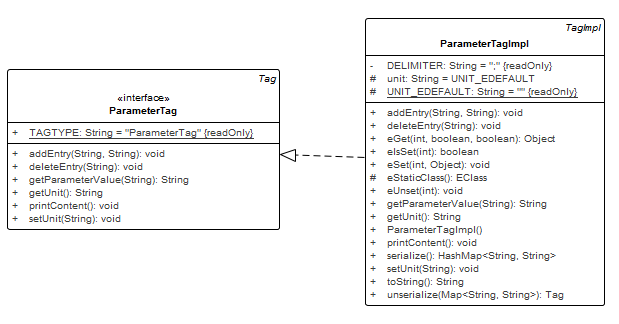
\includegraphics[scale=0.7]{ParameterTag.png}
  		  \caption{Darstellung der Klasse ParameterTagImplung das Interface ParameterTag}
     \label{uml.ParameterTag}
  \end{center}
\end{figure}






\subsubsection{ParameterTag}
Das Interface \textit{ParameterTag} dient als Schnittstelle für den Zugriff auf das Inhalt von ParameterTagImpl. Das Interface erweitert \textit{Tag}. Das \textit{Tag} Interface ist ein in TESTONA allgemein implementiertes Modell, welches auf ein Interface und eine implementierende Klasse basiert (siehe Kapitel \ref{sub.Tags}). In das Interface wird immer das Tagtyp definiert um \textit{Tags} voneinander unterscheiden zu können.

\begin{lstlisting}
public static final String TAGTYPE = "ParameterTag";
\end{lstlisting}

Das \textit{Tag} wurde um die in Abbildung \ref{uml.ParameterTag} zu sehende Methoden erweitert. 

\subsubsection{ParameterTagImpl}
Die Klasse \textit{ParameterTagImpl} erweitert die Klasse \textit{TagImpl} und implementiert \textit{ParameterTag}. In dieser Klasse werden die Vorteile von das Tagmodell deutlicher. Die Klasse \textit{TagImpl} definiert sehr nützliche Methoden und Eigenschaften die in \textit{ParameterTagImpl} weiter angewendet werden.\\

Jedes \textit{Tag} hat als Eigenschaft einen Namen. In diese Klasse entspricht der Name, ein Parametername der aus der Parametertabelle gelesen wurde. Weiterhin ist über \textit{ID} eine eindeutige Identifikationsnummer definiert, um \textit{Tags} des gleichen Typs voneinander zu unterscheiden. Es wurde ein weiteres Attribut implementiert, dass die Einheit (\textit{unit}) des Parameters definiert\\

Der Inhalt von das \textit{Tag} ist durch ein \textit{EcoreEMap<String, String>} definiert. Das erste String ist ein Schlüsselwert und das zweite String der Wert. Im diesem Fall ist der Schlüssel der Name einer Variante, und der Wert ist der Parameterwert des Parameters in dieser Variante. Der Inhalt und Struktur eines \textit{ParameterTags} sieht folgendermaßen aus:\\

\begin{table}[h]
\begin{center}
	\begin{tabular}{|l||ll|}
	 \hline
	 \multicolumn{3}{|c|}{ParameterTag}\\
	 \hline\hline
	 ID			& \multicolumn{2}{|c|}{30}\\
	 \hline
	 Name		& \multicolumn{2}{|c|}{max\_speed}\\
	 \hline
	 Unit		& \multicolumn{2}{|c|}{[km/h]}\\
	 \hline
	 \multirow{5}{*}{Content}	&Key			&Value\\ \cline{2-3}
	 							&Generic		&50\\
	 							&Cabrio		&100\\
	 							&Kombi		&200\\
	 							&Limo		&300\\
	 \hline
	\end{tabular}
	
	\caption{Beispiel eines ParameterTags}
	\label{table:ParameterTagStruktur}
\end{center}
\end{table}


Anhand der Methode \textit{getContent()} kann der Inhalt eines \textit{Tags} aufgerufen werden und mit der Methode \textit{addEntry()} werden Inhalte hinzugefügt. Das Gegenteil kann man mit der Methode \textit{deleteEntry()} erreichen. Wie die Methoden genauer angewendet werden, wird im Listing \ref{lst:CreateParamTag} gezeigt.\\


Sehr relevant sind die Methoden \textit{serialize()} und \textit{unserialize(Map<String, String>)} die für das Schreiben und das Lesen der .testona Datei zuständig sind. Zum Schreiben wird ein \textit{HashMap<String, String>} Objekt zurückgegeben. Das erste \textit{String} beinhaltet der Name des Parameters gefolgt von die Variantennamen. Die Werte sind durch ein Vereinbartes Trennzeichen (;)  getrennt. Das zweite \textit{String} beinhaltet die Einheit des Parameters und die Parameterwerte (in einer geordneten Reihenfolge). Der XML Eintrag für das obige Beispiel (Tabelle \ref{table:ParameterTagStruktur}) wurde wie folgt aussehen:\\

\begin{lstlisting}[caption={XML Darstellung eines ParameterTags}, captionpos=b]
<Tag id="30" type="ParameterTag">
	<Content key="max_speed;Generic;Cabrio;Kombi;Limo" value="km/h;50;100;200;300"/>
<Tag/>
\end{lstlisting}


Beim Laden der .testona Datei erkennt das Programm anhand des Attributs \texttt{type} um welches Typ von \textit{Tag} es sich handelt. Die Methode \textit{unserialize} bekommt als Eingansparameter die in \textit{serialize()} erstellte Zeile als ein \textit{Map<String, String>} Objekt. Durch das Trennzeichen werden die jeweilige Werten voneinander unterschieden und zu den zugehörigen Variablen (name, unit, content) zugeordnet. Beider Vorgänge funktionieren automatisiert dank der Vererbung.

%#######################################################################################
\subsection{ParameterManager}\label{sub:ParameterManager}

\begin{figure}[h!]
  \begin{center}
    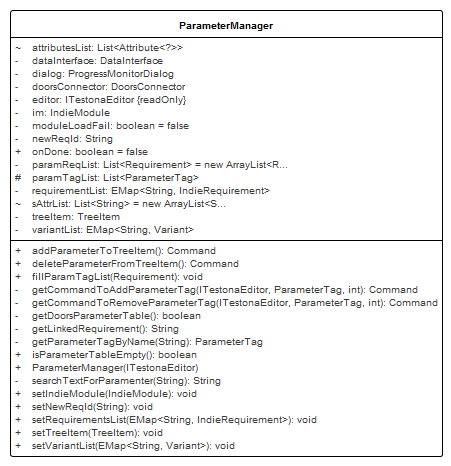
\includegraphics[scale=0.7]{KD_ParameterManager.png}
  		  \caption{Klasse ParameterManager}
     \label{kd.ParameterMananger}
  \end{center}
\end{figure}

Die Klasse \textit{ParameterManager} überprüft und startet die Parameterersetzung. Sie beinhaltet die private innere Klasse \textit{DoorsConnector}, diese kümmert sich um den Verbindungsaufbau mit DOORS und das Laden von den Parameterwerten aus der Parametertabelle. Die Klasse \textit{DoorsConnector} wird genauer in siehe Kapitel \ref{sub.DoorsConn} erklärt.\\


Mit dem Aufruf der Methode \textit{addParameterToTreeItem()} wird die Parameterersetzung gestartet. Die Methode hat als Rückgabewert ein Kommando, indem ein Parameter hinzugefügt oder gelöscht wird (siehe Kapitel \ref{sub.Command}). Als erstes überprüft die Methode ob die an das Baumelement verlinkte Anforderung ein Parameter beinhaltet. Falls kein Parameter in der Anforderung gefunden wurde, gibt die Methode den Wert \textit{null} zurück. Wenn ein Parameter gefunden wurde, wird der Name in einer Variablen gespeichert um es aus DOORS laden zu können. Wenn noch keine Parameter lokal zu Verfügung stehen (in Form von \textit{ParameterTag} innerhalb einer Liste) wird die Verbindung mit DOORS gestartet. Die erforderliche Angaben zum Verbindungsaufbau befinden sich in der Variable \textit{im} vom Typ \textit{IndieModul} (diese wurde von der Klasse \textit{VariantsManager} gesetzt aus das \textit{RequirementsConnectionTag}). Das Objekt der Klasse \textit{DoorsConnetor} hat Zugriff auf \textit{im} und kann die gespeicherte Daten abfragen.\\


Während die Verbindung entsteht und die Parametertabelle geladen wird, wird dem Benutzer ein Dialogfenster angezeigt. Dieser blockiert die Benutzeroberfläche und zeigt ein Fortschrittsbalken. Nach einem erfolgreichen Verbindungsaufbau wird die Parametertabelle geladen. Der Pfad zu der Parametertabelle in DOORS ist als Attribut des Hauptmoduls gespeichert. In das Objekt \textit{im} befindet sich der Pfad zum Hauptmodul. Die aktuell implementierte DOORS API in TESTONA kann nicht diese Attribute abfragen. Eine in Moment in Entwicklungszustand neue API wird in der Lage sein, die Attribute abfragen zu können. An dieser Stelle wurde als Kompromiss eine Konstante angelegt, in der sich der Pfad zur Tabelle befindet.\\

 
Wenn ein Parameter und die zugehörige Werte geladen worden sind, werden sie in \textit{ParameterTag} Objekt gespeichert. Die Methode \texttt{fillParamTagList(Requirement req)} agiert als Parser und wandelt der Übergabeparameter in ein ParameterTag. Zu beachten ist, dass innerhalb DOORS jede Zeile in ein Modul als eine Anforderung betrachtet wird. Danach wurde die Namensgebung vereinbart und der Übergabeparameter ist vom Typ \textit{Requirement}. In das \textit{Requirement} Objekt befinden sich die Variantennamen und die Parameterwerte. Der folgende Quelltextausschnitt kümmert sich im die Speicherung der Parameterwerte in ein \textit{ParameterTag}.\\


\begin{lstlisting}[caption={Auszug von der Erstellung der ParameterTags}, captionpos=b,label={lst:CreateParamTag}]
ParameterTag tempTag = new ParameterTagImpl();
		
for(int i = 0; i < attributesList.size(); i++){
	
	//An der nullte Stelle steht immer der Parametername
	if(i == 0) {
		tempTag.setName(req.getValue(attributesList.get(0)).getValueAsString());
	} else {
		//Füge ein Eintrag hinzu 
		tempTag.addEntry(sAttrList.get(i),
				req.getValue(attributesList.get(i)).getValueAsString());
	}
}
paramTagList.add(tempTag);
\end{lstlisting}


Die Variable \texttt{attributesList} beinhaltet die in DOORS definierten Varianten\footnote{Jede Variante in das DOORS Modul wird als ein Attribut definiert und in einer Spalte angezeigt. Wobei nicht jede Spalte des Moduls ein Attribut ist.}. Die Liste wird iteriert und die Werte werden in das \textit{ParameterTag} gespeichert. Zwei Attribute sind für jedes Parameter in der Liste mindestens definiert. Diese sind der Parametername und ein Standartwert. Möglicherweise ist auch die Einheit des Parameters definiert. Die geladene Werte werden kontrolliert ob sie ungleich ein leerer \textit{String} sind\footnote{Im Ladevorgang einer Anforderung und ihre Attribute in DOORS, wird nicht zwischen leeren und befüllte Zellen unterschieden. Der Rückgabewert ist immer ein \textit{String}. Wenn die Zelle leer ist, wird ein leerer \textit{String} zurückgegeben.}, bevor sie in ein \textit{ParameterTag} gespeichert werden.\\


Wenn alle vorhandenen Varianten für dieses Parameter iteriert worden sind, wird überprüft ob der Inhalt (die Variable \textit{content} des \textit{ParameterTags}) der temporären Variable \texttt{tempTag} nicht leer ist. Es kann vorkommen, dass ein Parameter in das Modul definiert ist, aber keine weitere Informationen wurden ausgefüllt. Wenn Inhalte vorhanden sind, wird das \textit{ParameterTag} zur eine Liste von \textit{ParameterTags} hinzugefügt.\\

Nachdem die Parameter geladen werden konnten und die Liste befühlt ist, wird die Verbindung mit DOORS geschlossen. Das Dialogfenster wird danach geschlossen und die Benutzeroberfläche wird freigegeben. Während dessen wird ein der Liste das richtige \textit{ParameterTag} geladen und die Methode \textit{getCommandToAddParameter()} wird aufgerufen. Diese Methode erzeugt ein Objekt der Klasse \textit{AddParameterTagCommand}. Das zurückgegebene Kommando wird an die Klasse \textit{VariantsManager} weitergeleitet, die wiederum das Kommando an das \textit{ResourSetListener} weitergibt. Dort wird das Kommando verarbeitet.\\


Für den Fall, dass eine Anforderung aus ein Baumelement gelöscht wird, muss zuerst überprüft werden ob die Anforderung ein Parameter beinhaltet. Wenn ein Parameter gefunden worden ist, wird das \textit{ParameterTag} aus dem Baumelement geladen. Mithilfe der Klasse \textit{RemoveParameterTagCommand} wird das \textit{ParameterTag} aus dem Baumelement entfernt.

%#######################################################################################
\subsection{Kommandos}\label{sub.Command}
Für das Hinzufügen bzw. Löschen eines Parameters in einem Baumelement wurden zwei Klassen implementiert, dass aus die Klasse \textit{RecordingCommand} erben. Die Klasse \textit{RecordingCommand} ist eine partielle Implementierung der Klasse \textit{Command}. Diese Klasse nimmt die  Manipulierung der Objekte der Subklasse auf und erzeugt daraus ein Kommando\footnote{14.02.2015; http://download.eclipse.org/modeling/emf/transaction/javadoc/ 1.2.3/org/eclipse/emf/transaction/RecordingCommand.html}. Eine der implementierten Klassen erzeugt ein Kommando für das Hinzufügen eines \textit{ParameterTags} an einem Baumelement\footnote{AddParameterTagCommand}, während der zweiten für das Löschen zuständig ist\footnote{RemoveParameterTagCommand}. Der Konstruktor der beiden Klassen haben die gleichen Parametern. Es werden der aktuelle Editor-Objekt übergeben, sowie das Baumelement ID und das \textit{ParameterTag}.\\


Die Methode \textit{doExecute()} wird überschrieben um die Änderung vorzunehmen. Als erstes werden alle Baumelemente geladen und iteriert bis das Baumelement gefunden wird, dass benötigt wird (anhand er ID). Soll ein \textit{ParameterTag} hinzugefügt werden, dann wird die Methode \textit{addTag(ParameterTag pTag)} aufgerufen.\\


Soll eine \textit{ParameterTag} gelöscht werden, dann wird die Methode \textit{removeTag(ParameterTag pTag)} aufgerufen. Danach muss auch der Name des Baumelementes neu gesetzt werden. Wenn ein Baumelement ein Parameter besitzt, je nach aktive Variante, wird die Darstellung geändert (siehe Kapitel \ref{sec.visialisierung}). Dafür wird der Name des Baumelementes geladen und falls eine Rücksetzung nötig ist, wird diese gemacht. Genaueres dazu wird in Kapitel \ref{sec.LoesungVisualisierung} veranschaulicht.\\

%#######################################################################################
\subsection{Die DOORS Verbindng}\label{sub.DoorsConn}
\subsubsection{DoorsConnector}
%\begin{figure}[h!]
%  \begin{center}
%    \includegraphics[scale=0.7]{.jpg}
%  		  \caption{Darstellung der innere Klasse DoorsConnector in UML}
%     \label{ttn.DoorsConnetor}
%  \end{center}
%\end{figure}

Die private innere Klasse \textit{DoorsConnector} baut die Verbindung zwischen den TESTONA und DOORS auf. Sie implementiert das Interface \textit{IConnectionListener}, dass ein \textit{Listener} für die Verbindung - Events umfasst. Für das Laden von Dateien aus DOORS benötigt die Klasse noch ein \textit{Listener} (IDataListener) und ein \textit{Adapter}(IReqLoadAdapter) \\

Als erstes wird von der Klasse \textit{ParameterManager} die Methode \textit{connectToDoors()} aufgerufen. Diese baut die Verbindung auf, indem gespeicherte Verbindungsdaten aufgerufen werden. Wie bereits in Kapitel \ref{sub:ParameterManager} erwähnt, beinhaltet eine Anforderung die Informationen wo die Anforderung gespeichert ist (welches DOORS Modul und über welches Interface das Modul zu erreichen ist). Für den Verbindungsaufbau werden folgende Objekte benötigt:

\begin{itemize}
\item \textbf{DataInterface: }Über diese Klasse erfolgt die Datenanfrage an DOORS. Die Verbindung wird aufgebaut sowie getrennt. Es werden als erstes die Ordner geladen, danach einzelne Projekte und die nötige Module. Es können verschiedene Darstellungen der Module auch geladen werden (diese müssen in DOORS definiert sein). Hier werden auch direkt einzelne Anforderungen angefragt. Relevant für diese Arbeit ist, dass hiermit das Modul Parametertabelle in DOORS geladen wird.

\item \textbf{PreferenceManagment: } Hier werden die in TESTONA gespeicherte Verbindungsdaten behandelt. Es können Microsoft Access Verbindungensdaten gespeichert werden, aber wir werde nur DOORS betrachten.

\item \textbf{Connector: }beschreibt eine einzelne Verbindung, hat ein \textit{DataIterface}- und \textit{PreferenceManagmentobjekt}

\item \textbf{ConnectionManager: }Singleton. Die Klasse handelt aktive und offene Verbindungen. Hier werden die \textit{ConnectionListeners} und das \textit{DataInterface} für den richtigen \textit{Connector} geregelt.

\end{itemize}


Um die Verbindung mit DOORS aufzubauen muss als erstes die Instanz des \textit{ConnecionManagers} lokal referenziert werden (weil es ein \textit{Singleton} ist, darf kein neues Objekt erzeugt werden). Wenn die Instanz des \textit{ConnectionManagers} geladen ist, kann jetzt der \texttt{connector} aus dem \textit{ConnectionManager} aufgerufen werden.

\begin{lstlisting}[caption={Verbindungsaufbau}, captionpos=b]
try {
	connector = ConnectorManager.getInstance()
				.getConnector(im.getInterId());
	dataInterface = conManager.getNewDataInterface(connector, this);
} catch (ExtensionException e) {
	e.printStackTrace();
}
\end{lstlisting}

 Um dem richtigen \texttt{connector} aufzurufen muss aus das \textit{IndieModul} (\texttt{im.getInterId()}, siehe Kapitel \ref{sub.VariantsManager}) die Interfacekennung als Übergabeparameter angegeben werden. Als nächstes kann über den \textit{ConnectionManager} eines neues \textit{DataInterface} erzeugt werden, wo der \texttt{connector} und das aktuelle Objekt (\textit{DoorsConnector}) übergeben werden.\\
 
Aus den in TESTONA gespeicherte Verbindungspräferenzen werden die Verbindungsparameter für DOORS geladen. An dieser Stelle braucht das \textit{DataInterface} die nötige \textit{Listeners} bevor die Verbindung aufgebaut wird. Durch die Methode \textit{addListener(listener)} wird das \textit{RequirementDataListener} und das \textit{IConnectionListener} (von \textit{DoorsConnetor} implementiert) gesetzt. Mit dem Aufruf der Methode \textit{connecteInterface(Verbindungsparameter)} wird das \textit{DataInterface} an DOORS verbunden.\\

Der Grund warum ein \textit{IConnectionListener} implementiert wird, lautet dass der Verbindungsaufbau in einem neuen Thread stattfindet. Das \textit{DoorsConnetor} Objekt wird über das \textit{IConnectionListener} benachrichtigt ob die Verbindung stattgefunden hat. Die Methode\texttt{interfaceConnected} (aus dem \textit{IConnectionListener}) wird aufgerufen, wenn die Verbindung erfolgreich entstanden ist.

\begin{lstlisting}[caption={Verbindungsaufbau war erfolgreich}, captionpos=b]
@Override
public void interfaceConnected() {
	connected = true;
	reqDataListener.setListener(reqLoadListener);
	dataInterface.loadModule(PARAM_PATH, this, false);
}
\end{lstlisting}

Der gesetzte \textit{RequirementDataListener} benötigt ein \textit{RequirementLoadListener}, dass eine rückmeldung gibt, wenn die Zeilen aus einer Tabelle fertig geladen worden sind. Die Tabelle wird anhand der Methode \texttt{loadModule} wird ein DOORS Modul (Tabelle) geladen. Welches Modul geladen wird, spezifiziert der Parameter \texttt{PARAM\_PATH}. Es gibt an wo sich das Modul in der DOORS Datenbank befindet. Der \textit{RequirementDataListener} erhält die Nachricht, dass ein Modul geladen worden ist. Weiter dazu wird im Kapitel \ref{sub.RequirementDataListener} erläutert.\\


Es wird angenommen, wenn der Benutzer die Parameterersetzung für ein Parameter wahrnimmt, dass er es für weitere Parameter wahrnehmen wird. Da die Datenmenge von einer Parametertabelle relativ gering ist, wurde hier, bezüglich der offene Frage bei dem Lösungsansatz (siehe Kapitel \ref{sec.parameterspeicherung}), die Parametertabelle komplett importiert. 
Ein weiterer Grund lautet, dass nicht für jeder Parameter erneut eine DOORS Verbindgun enstehen muss. So wird die Rechen- und Reaktionszeit von TESTONA so weit es geht gering gehalten. Die Parametertabelle wird erst bei der Verknüpfung von einer Anforderung mit einem Baumelement importiert und nicht beim Import der Anforderungen. 

Wenn die Parametertabelle komplett geladen wurde, ermöglicht die Methode \textit{closeConnection} die Verbindung mit DOORS zu beenden und das \textit{DataInterface} zu schließen.





\subsubsection{RequirementDataListener}\label{sub.RequirementDataListener}

Ist ein Event-Listener, dass auf die Rückmeldung vom Laden eines Moduls wartet. Relevant ist die Methode \texttt{onModuleLoad} die die Zeilen aus der Tabelle liest und speichert.\\

\begin{lstlisting}[caption={Laden der Parametertabelle nach Zeilen}, captionpos=b]
@Override
public void onModuleLoad(Module module, Object family, boolean reload){

	BasicRequirement baseReq;
	saveAttributesNames(module);
				
	for (String reqId : module.getRequirementIds()) {

		baseReq = dataInterface.getRequirement(module, reqId,
				reqLoadListener);

		if (baseReq.checkStatus(BasicRequirement.STATUS_LOADED)){
			paramReqList.add((Requirement) baseReq);
			fillParamTagList((Requirement) baseReq);
		}
	}
	dataInterface.flush(reqLoadListener);
}
\end{lstlisting}

Zu beachten ist, dass in DOORS jede Zeile in einer Tabelle als eine Anforderung (eng. Requirement) gesehen wird. Daher heißen Variablen und Methoden oft \glqq Requirement\grqq~ oder Abkürzung des Wortes (req). Die Methode \texttt{saveAttributesNames} speichert die im geladenes Modul vorhandenen Attribute. Im diesem Fall (treu zum Beispiel mit dem Auto) sind es:

\begin{itemize}\itemsep1pt
\item Paramenter Name
\item Default Value
\item Cabrio Value
\item Kombi Value
\item Limo Value
\end{itemize}

Diese Attribute repräsentieren die Varianten und ein Standardwert, sowie der Name des jeweiligen Parameter. In der Schleife werden alle Zeilen im Modul iteriert und geladen. Wenn die Zeile (\texttt{baseReq}) vollständig geladen wurde, wird diese in der globalen Liste \texttt{paramReqList} als ein \texttt{Requirement} Objekt gespeichert. Die Methode \texttt{fillParamTagList} erzeugt die \textit{ParameterTags} und wurde in Kapitel \ref{sub:ParameterManager} erläutert.\\

Wenn eine Zeile nicht vollständig geladen werden konnte, gibt es das \textit{RequirementLoadListener}, dass sich um das vollständige laden der Zeilen kümmert. Das \textit{RequirementLoadListener} wird in dieser Klasse instantiiert und von der \textit{DoorsConnetor} Klasse gesetzt. Weiter dazu im nächsten Kapitel.


\subsubsection{RequirementLoadListener}\label{sub.RequirementLoadListener}
Der \textit{RequirementLoadListener} reagiert wenn eine Zeile nicht völlstandigt geladen worden ist, und wartet bis diese geladen wird. Die Methode \texttt{onLoad} bekommt als Eingabeparameter eine Liste der nicht geladenen Zeilen.

\begin{lstlisting}[caption={Nachladen der Parametertabelle nach Zeilen}, captionpos=b]
public void onLoad(List<BasicRequirement> requirements) {

	for (BasicRequirement baseReq : requirements) {
		paramReqList.add((Requirement) baseReq);
		fillParamTagList((Requirement) baseReq);
		
	}
}
\end{lstlisting}

Diese Liste wird iteriert und wie in \textit{RequirementDataListener} in der globalen Liste \texttt{paramReqList} als ein \texttt{Requirement} Objekt gespeichert.\\

Weiterhin meldet diese Klasse wenn alle Zeilen aus das DOORS Modul geladen wurden. Das wartenden Dialogfenster aus \ref{sub:ParameterManager} wird benachrichtigt, dass es geschlossen werden kann. Die Benutzeroberfläche von TESTONA ist somit wieder für den Benutzer erreichbar.



%#######################################################################################
%#######################################################################################
\newpage
\section{Darstellung der Parameterwerte}\label{sec.LoesungVisualisierung}
\paragraph{}

Nachdem Parameter in Baumelement vorhanden sind, sollten die Werte angezeigt werden. Wenn ein Pfeil oder die Kombo-Box (siehe Kapitel \ref{sec.visialisierung}) für eine Änderung der Variantenansicht betätigt wird, muss für jedes Baumelement überprüft. Es wird überprüft, ob für die aktive Variante ein Parameterwert definiert worden ist.\\

In \textit{VariantsManager}\\

 \textit{setNamesWithValues} \\
 \textit{executeEMFCommand} \\
 \textit{RenameTreeItemCommand}\\
 \textit{arrangeAll}\\
 
 


%#######################################################################################
%#######################################################################################
\newpage
\section{Testfallgenerierung und Optimierung}
\paragraph{}
Erläuterung der Lösungen zu 4.3
\chapter{Evaluierung}\label{chp:Evaluierung}
\paragraph{}

Als letzter Schritt für die Beendigung der Entwicklung des Testprogrammes müssen Test durchgeführt werden und die Ergebnisse evaluiert werden.


%#######################################################################################
%#######################################################################################
\newpage
\section{Testaufbau und -Ablauf} \label{sec:test}
\paragraph{}
Um das Programm evaluieren zu können müssen verschiedene Tests durchgeführt werden. Für die Tests wurden das Programmierte nach Aufgabe geteilt:

\begin{enumerate}
\item Listeners
\item DOORS Verbindung und Import der Parameter
\item Speichern der Parameter
\item Darstellung der Parameter
\item Löschen von Parametern
\item Lesen und Schreiben der TESTONA Datei
\end{enumerate}


\subsubsection{Listeners}
Die Erweiterung des \textit{ResourceSetListeners} wurde getestet, indem alle reinkommende Nachrichten mit Hilfe des Debuggers überprüft worden sind. Da das \textit{Listener} erweitert wurde, muss überprüft werden, dass die Erweiterung die anderen Funktionalitäten nicht negativ beeinflussen. Dafür wurde mit dem Debugger Schritt für Schritt überprüft, dass der neu implementierte Quelltext nur in den richtigen Fällen aufgerufen wird. Die Fälle sind das Löschen oder das Hinzufügen eines \textit{ParameterTags} zu einem Baumelement.\\



\subsubsection{DOORS Verbindung und Import der Parameter}
Da die Bibliothek for die DOORS Verbindung schon existierte und bereits getestet war, muss hier nur die Funktionalität dieser überprüft werden. Es wurden Negativtest\footnote{Reaktion des Programms auf eine falsche Eingabe.} durchgeführt. Die Negativtest bestanden aus falsche Log-in Parameter für die DOORS Datenbank. Dabei wird der Benutzer aufmerksam gemacht, dass die Verbindung nicht entstehen konnte. Dieser Fall sollte eigentlich nicht auftreten, da die Log-in Daten in TESTONA gespeichert worden sind. Wären diese falsch, hätte der Benutzer es bei dem Import der Anforderungen bemerkt.\\


Weiterhin wurden das Öffnen und Schließen der DOORS Module getestet und der Verbindungsaufbau und - Abbau. Dabei wurde überprüft, dass die Verbindungen richtig getrennt worden sind. Nach das Öffnen der DOORS Module wurde auch überprüft, ob die Parameterwerte richtig in TESTONA gespeichert werden konnten. Hier wurde Positiv\footnote{Reaktion des Programms auf eine (nach den Anforderung) richtige Eingabe.} - und Negativtest durchgeführt. Für die Positivtest wurden plausible Werten in die Parametertabelle eingetragen. In den Negativtest wurden Zellen leer gelassen oder mit Escape - Sequenzen (\textbackslash n, \textbackslash r oder \textbackslash b) befüllt. Dabei musste das Programm erkennen, dass die Zelle kein Wert beinhaltete. Als richtige Werte werden Buchstaben, zahlen und Sondereichen bewertet.\\



\subsubsection{Speichern der Parameter}
Die Speicherung der Parameter in TESTONA musste an zwei Stellen getestet werden. Die erste Stelle ist nach dem Import der Parametertabelle und die Erstellung der \textit{ParameterTags}. Hier wurde überprüft, dass die in die Parametertabelle eingegebene Werte richtig in TESTONA übernommen worden sind. Weiterhin mussten die Werte in der richtigen Reihenfolge in das \textit{ParameterTag} Objekt gespeichert und dargestellt werden. Die Escape - Sequenzen und leeren Zellen sollten ignoriert werden.\\


Die zweite Stelle an der die Parameterspeicherung getestet werden musste, ist bei das Speichern eines Parameters in einem Baumelement. Als erstes musste getestet werden, dass das \textit{ParameterTag} an das Baumelement hinzugefügt worden ist. Parallel dazu wurden das richtige Ausfuhren des \textit{AddParameterTagCommand} Kommandos getestet. Weiterhin musste auch betrachtet werden, dass ein \textit{ParameterTag} in einem Baumelement mehrere Parameter beinhalten kann. Hier wurde auch getestet, dass der \textit{ParameterTag} richtig die verschiedene Parameter mit dem zugehörigen Varianten und Parameterwerten speichert.\\



\subsubsection{Darstellung der Parameterwerte}
Bei der Darstellung der Parameterwerte muss geachtet werden, dass der richtige Parameterwert angezeigt wird. Je nach aktive Variante muss das Programm der richtige Wert aus das \textit{ParameterTag} lesen und darstellen. Oder wenn kein Wert zur Verfügung stand, dass nur der Name des Baumelements angezeigt wurde. Hier wurde das \textit{ParametarTag} Objekt mit der Ausgabe im TESTONA Editor verglichen.\\


\subsubsection{Löschen von Parametern}
Wie bei das Speichern von Parametern gibt es hier auch zwei Fälle die betrachten werden müssen. Der erste Fall ist, wenn ein \textit{ParameterTag} aus ein Baumelement gelöscht werden muss. Hier wird auch parallel das Ausführen des \textit{removeParameterTagCommand} Kommandos getestet. Dabei muss das \textit{ParameterTag} aus das Baumelement gelöscht werden.\\


Der zweite Fall ist, wenn ein Parameter aus ein \textit{ParameterTag} gelöscht werden muss (in das \textit{ParameterTag} befinden sich mindestens zwei verschiedene Parameter). Hier musste beachtet werden, das nur der richtige Eintrag entfernt wurde. Falls nach das Entfernen des Parameters, das \textit{ParameterTag} nur noch ein Parameter beinhaltete, muss die Struktur des \textit{ParameterTags} umgestellt werden.\\


\subsubsection{Lesen und Schreiben der TESTONA Datei}
Das letzte wichtige Aspekt das noch getestet werden muss, ist das Schreibe und Lesen der TESTONA Datei. Wenn der Benutzer Parameter importiert und an Baumelement verknüpft hat, müssen diese in der TESTONA Datei gespeichert werden. Dafür wurde den Inhalt von das \textit{ParameterTag} Objekt mit das XML - Eintrag der TESTONA Datei verglichen.\\


Wenn das Speichern erfolgreich war, muss das Lesen getestet werden. Dafür wurde den Inhalt des erzeugten \textit{ParameterTags} mit dem Eintrag in der XML Datei gegenüber gestellt.



%#######################################################################################
%#######################################################################################
\newpage
\section{Ausfallrisiko}
\paragraph{}
Nachdem alle in Kapitel \ref{sec:test} Tests erfolgreich durchgeführt worden sind, entsteht immer noch ein Ausfallrisiko. Der neue Quellcode befindet sich in der \textit{pre - Alpha} Version. Das Bestehen der durchgeführte Tests ergibt die erste Alpha Version\footnote{Erste nicht vom Entwickler durchgeführte Tests} des Programmes.\\


Die programmierten Erweiterungen von TESTONA basieren nicht auf das sogenannte \glqq vier Augen Prinzip\grqq~ und da Programm kann noch Fehler beinhalten. Da nur der Entwickler bis jetzt die neue Erweiterung getestet hat, kann die Objektivität der Tests nicht gewährleistet sein. An dieser Stelle müssen genauere White - Box Tests erstellt und durchgeführt werden. Als nächstes Schritt müssen die Black - Box Tests erfolgen.\\


Ein weiterer Punkt für das Ausfallrisiko ist, dass die durchgeführten Tests auf einfache Beispiele basieren. Das heißt die Klassifikationsbäume und Parametertabelle recht simpel und klein waren. Es ist nötig durchaus komplexere Beispiele zu betrachten, indem der Klassifikationsbaum aus mehrere Klassen und Klassifikation besteht. Sowie die Parametertabelle viele Parameter definiert. Aus der Grundlagen der Kombinatorik (siehe \ref{ssec:KM}) ist klar geworden, dass Fehlverhalten nicht unbedingt aus einzelnen falschen Parameter entstehen, sondern oft aus die Interaktion verschiedener Parameter.


%#######################################################################################
%#######################################################################################
\newpage
\section{Bekannte Fehler}
\paragraph{}
Nach der Durchführung der in Kapitel \ref{sec:test} worden verschiedene Fehler behoben. Bis jetzt ist nur noch ein Fehler bekannt, der nicht behoben werden konnte. Nachdem sich das Programm erfolgreich mit DOORS verbinden kann, konnte die Verbindung nicht richtig getrennt werden. Zwar versucht das Programm die Verbindung zwei Mal zu trennen. Im ersten Versuch wird die Verbindung erfolgreich getrennt und geschlossen. Aus bis jetzt unbekannten Gründen versuch das Programm ein zweites Mal die Verbindung zu DOORS zu trennen. Hier ersteht der Fehler, dass das \textit{ConnectionInterface} für die Verbindung nicht mehr zu Verfügung steht.\\


Nach mühsames suchen und Debuggen mithilfe von ein Mitarbeiter, konnten wir die Ursache des Fehlverhaltens nicht finden. Dieser Fehler wurde mit einer niedrigen Priorität versehen, da in der nähre Zukunft die DOORS API durch eine neuere ersetzt wird. Dabei wird der Quellcode für die Verbindung, Import und Trennung der DOORS Datenbank überarbeitet. Es ist sehr wahrscheinlich, dass dabei dieser Fehler behoben wird. Weiterhin bringt dieser Fehler TESTONA nicht zum Absturz. 
\input{7_Something/something.tex}
\chapter{Zusammenfassung und Ausblick}\label{chp:zusammenfassung}
%Lehnen Sie sich zurück von Ihrem Terminal und versuchen ein wenig Abstand zu den vielen Detail-Problemen Ihrer Diplomarbeit zu gewinnen:
%Was war wirklich wichtig bei der Arbeit? 
%Wie sieht das Ergebnis aus?
%Wie schätzen Sie das Ergebnis ein?
%Gab es Randbedingungen, Ereignisse, die die Arbeit wesentlich beeinflußt haben?
%Gibt es noch offene Probleme?
%Wie könnten diese vermutlich gelöst werden?\\\\



%#######################################################################################
%#######################################################################################
\newpage
\section{Optimierungskriterien}
\paragraph{}
%Testablauf optimieren in Betrachtung auf nur gültige Baumelemente in einer Variante und mögliche Testduplikate,

\paragraph{}


%##################################################################
% Abbildungsverzeichnis
%##################################################################
\listoffigures 

%##################################################################
% Listingsverzeichnis
%##################################################################
\lstlistoflistings


%##################################################################
% Anhang
%##################################################################

\begin{appendix}
	%%
%% Beuth Hochschule für Technik --  Abschlussarbeit
%%
%% Anhang
%%
%%%%%%%%%%%%%%%%%%%%%%%%%%%%%%%%%%%%%%%%%%%%%%%%%%%%%%%%%%%%%%%%%%%%%

\chapter{Anhang}

		
\section{CD}
Inhalt:
\begin{itemize}
\item Quellen
\item PDF-Datei dieser Arbeit
\end{itemize}

\newpage


\section{code 1}\label{code1}
\begin{lstlisting}	
hier kommt java code
\end{lstlisting}	


%****************************************************************************************
\newpage
%****************************************************************************************
\section{code 2}\label{code2}

		
\begin{lstlisting}	
hier kommt auch java code

\end{lstlisting}
\end{appendix}


%##################################################################
% Literaturverzeichnis
%##################################################################

%\nocite{*}
\clearpage\newpage
\addcontentsline{toc}{chapter}{Literatur- und Quellenverzeichnis}
\bibliographystyle{plain}
\bibliography{bhtThesis}

\end{document}  